

\chapter{Statistical interpretation and results}
\label{sec:results}

\section{Signal determination}
The signal efficiency of the selection is evaluated as the ratio between the number of selected events in each of the six channels (electron and muon channels, 0-, 1-, and 2-btag categories) under study and the total number of generated events in the Monte Carlo samples.  The signal efficiency as a function of the Higgs mass is fitted to a polynomial in order to be estimated for those Higgs mass hypothesis where no Monte Carlo sample is available, 
%as shown in Figure~\ref{fig:lineshape}.
as shown in Figure~\ref{fig:effvsmass}.

The narrow width approximation breaks down at high Higgs mass (typically $>400 GeV$) due to the very large Higgs width ($>70 GeV$). 
A more correct approach to describe the Higgs invariant-mass distribution has been proposed, known as Complex Pole Scheme (CPS)~\cite{Goria:2011wa}.
The total Higgs production cross section has been recomputed by the Higgs Cross Section Working Group to include the corrections due to CPS at high Higgs mass~\cite{LHC-HCS}.  In this analysis the simulated signal samples are properly re-weighted to follow the CPS.

At high Higgs mass the interference between the Higgs signal and the $gg\rightarrow ZZ$ background becomes large~\cite{Passarino:2012ri}.  The effect of interference has been shown to be constructive below the Higgs mass peak and destructive above. It therefore has a negligible effect on the total cross section (1-2\%) but it biases the ZZ invariant-mass distribution. Moreover the interference has been computed only at LO (leading order) while the signal is known at NNLO (next to next to leading order). In this analysis the uncertainty due to missing higher perturbative order on the interference and the simulated line-hape is also corrected in the re-weighting~\cite{Passarino:2012ri}.

After this is done, the obtained distribution should reflect the expectation for the Higgs events, both in yield and shape. This re-weighting has been included in the analysis in order to account for the correct distributions.

%%%%%%%%%%%%%%%%%%%%%%%
\begin{figure}[htbp]
\begin{center}
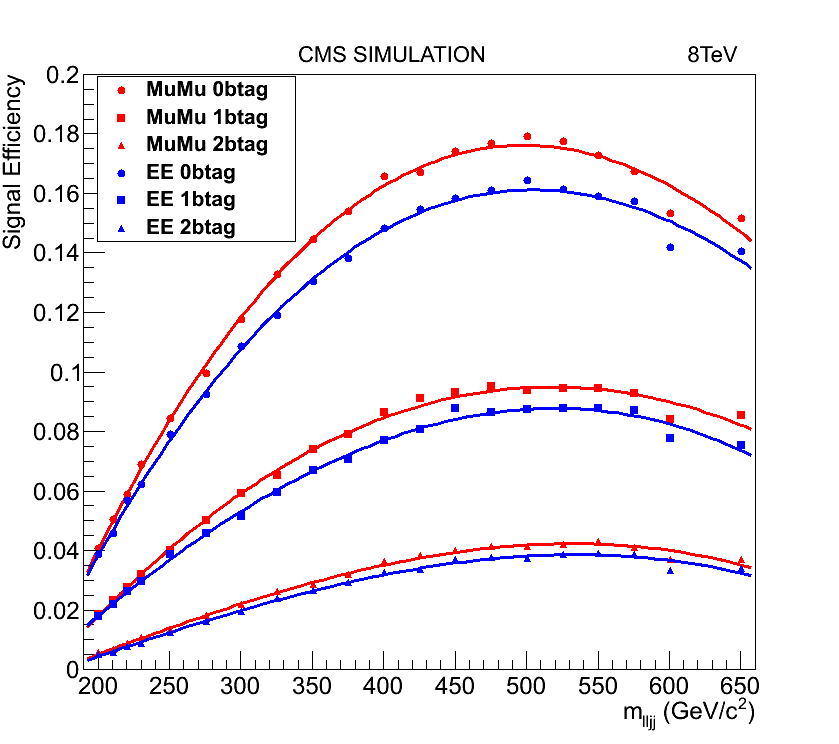
\includegraphics[width=0.49\textwidth]{plots/all_signal_effs.png}
\caption{
Parameterization of signal efficiency as a function of Higgs mass hypothesis in
0-btag (left), 1-btag (middle), 2-btag (right) categories and in the
muon (top) and electron (bottom) channels.
}
\label{fig:effvsmass}
\end{center}
\end{figure}


\section{Results}

Since the decay products of the Higgs boson can be fully reconstructed, it is possible to use the reconstructed Higgs boson mass distribution to discriminate Higgs signal events against background events. The reconstructed mass will peak around the true Higgs boson mass, $m_{H}$, for the signal, while for background processes it will have a broader distribution.  Consequently, a shape-based treatment of the expected and observed distribution of the invariant mass of the Higgs candidate (i.e. the 4-object mass) increases the sensitivity of the analysis, compared to a simpler counting experiment. Since the expected shape of the background and the signal cannot be obtained from first principles, an analytic function cannot be used. Therefore, a binned histogram-based calculation has been used for the shape analysis.

The normalization of the simulated background (Z+jets and diboson) in the signal region is allowed to vary.  The constraints come from the number of events in the $m_{jj}$ sideband in data. The signal-free regions of the $\mlljj$ distribution impose an additional constraint to the background normalization. The observed and expected numbers of events in the sideband region are given as input to the limit calculation tool. The calculation to discriminate signal from background events is performed independently for the six individual analysis channels (electrons and muons in the 0, 1, and 2-btag categories), and then combined taking into account the correlations among the systematic uncertainties. These uncertainties may affect either the shape of the distributions or their normalization, and are properly taken into account in the statistical analysis.

The mass distributions of the $\LL jj$ system are depicted in Figures~\ref{fig:ichepllqq} and~\ref{fig:ichepllqqLOG} for data in the signal region. The statistical uncertainty on the background is much smaller than the statistical uncertainty on the data, as the number of Z+jets simulated events used to estimate this background corresponds to a luminosity from 5 to 10 times larger. The full dataset (19.6~\fbinv{}) is used to assess the good modeling of the background in the $m_{jj}$ sideband region (Figures~\ref{fig:llqqSB} and~\ref{fig:llqqSBLOG}). Residual differences are taken as a systematic uncertainty, as explained in the previous section. As a cross check, the $\mlljj$ distributions for the electron and muon channels are studied separately, both in the $m_{jj}$ sideband and signal regions.  They show an excellent agreement as can be seen in Appendix~\ref{sec:emuratios}.

%%%%%%%%%%%%%%%%%%%%%%%%%%%%%%%%%%%%%%%%%
\begin{figure}[htb]
\begin{center}
\centerline{
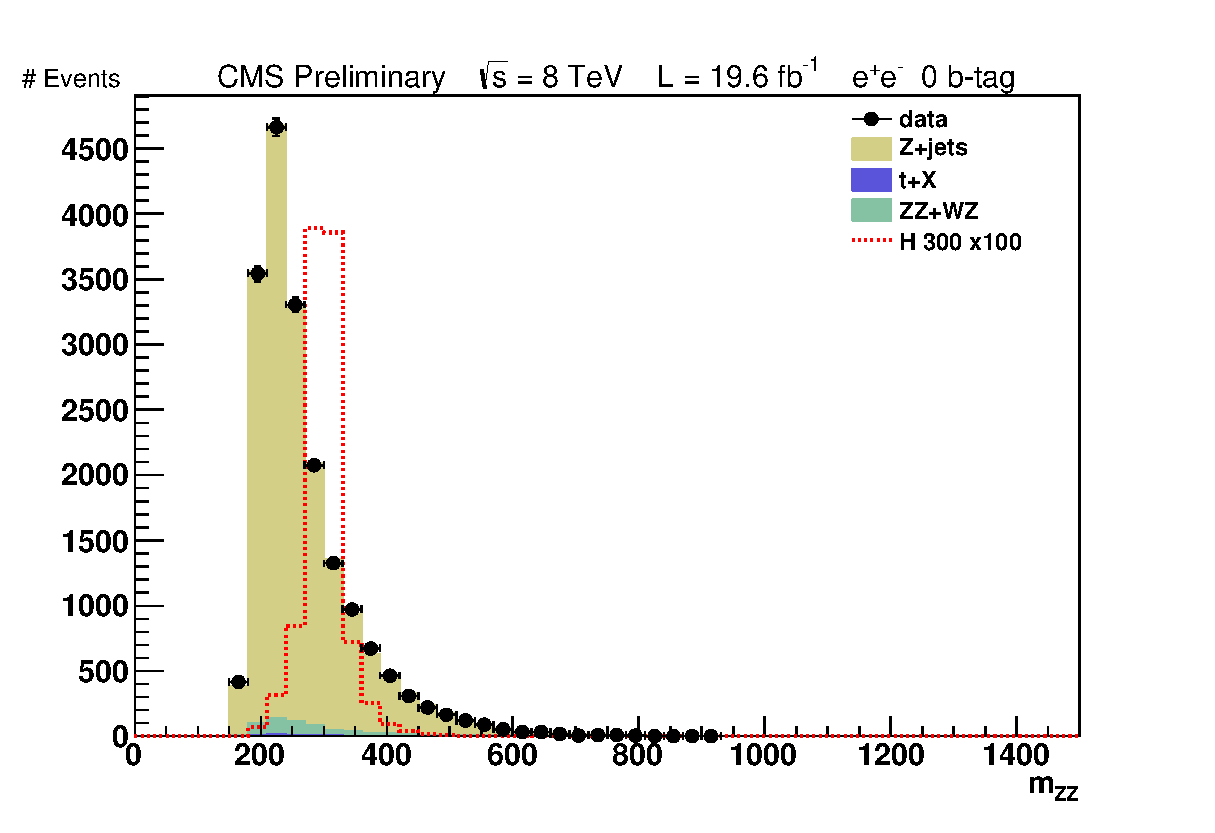
\includegraphics[width=0.33\textwidth]{presentation/defense/images/final/0/el/mZZ_signal.eps}
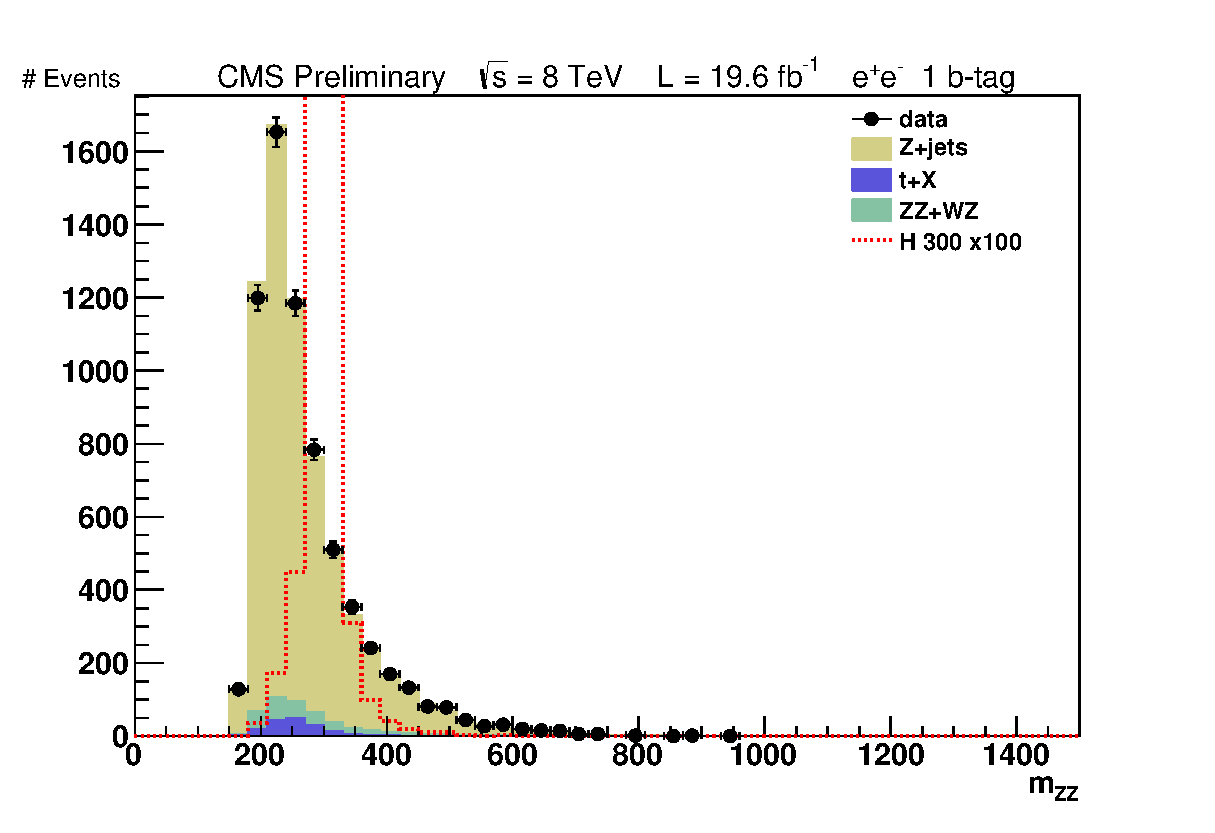
\includegraphics[width=0.33\textwidth]{presentation/defense/images/final/1/el/mZZ_signal.eps}
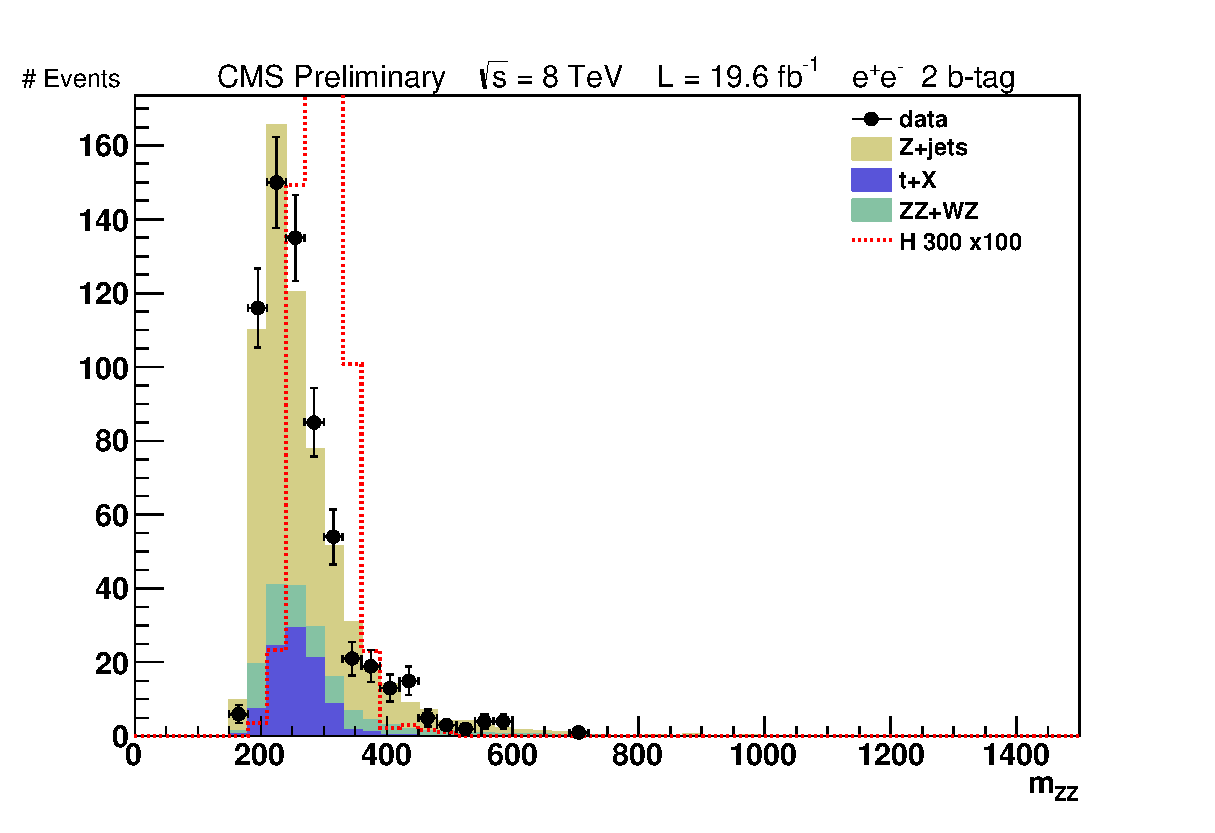
\includegraphics[width=0.33\textwidth]{presentation/defense/images/final/2/el/mZZ_signal.eps}
}
\centerline{
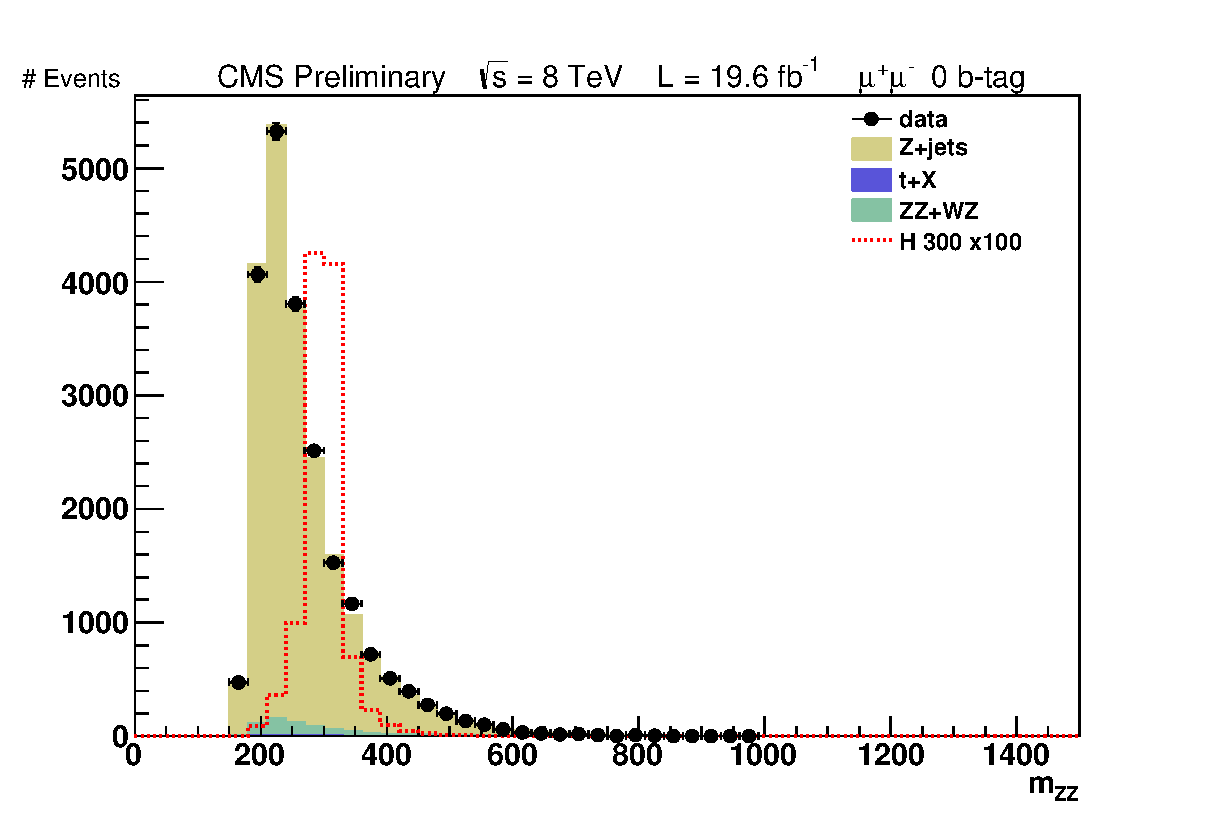
\includegraphics[width=0.33\textwidth]{presentation/defense/images/final/0/mu/mZZ_signal.eps}
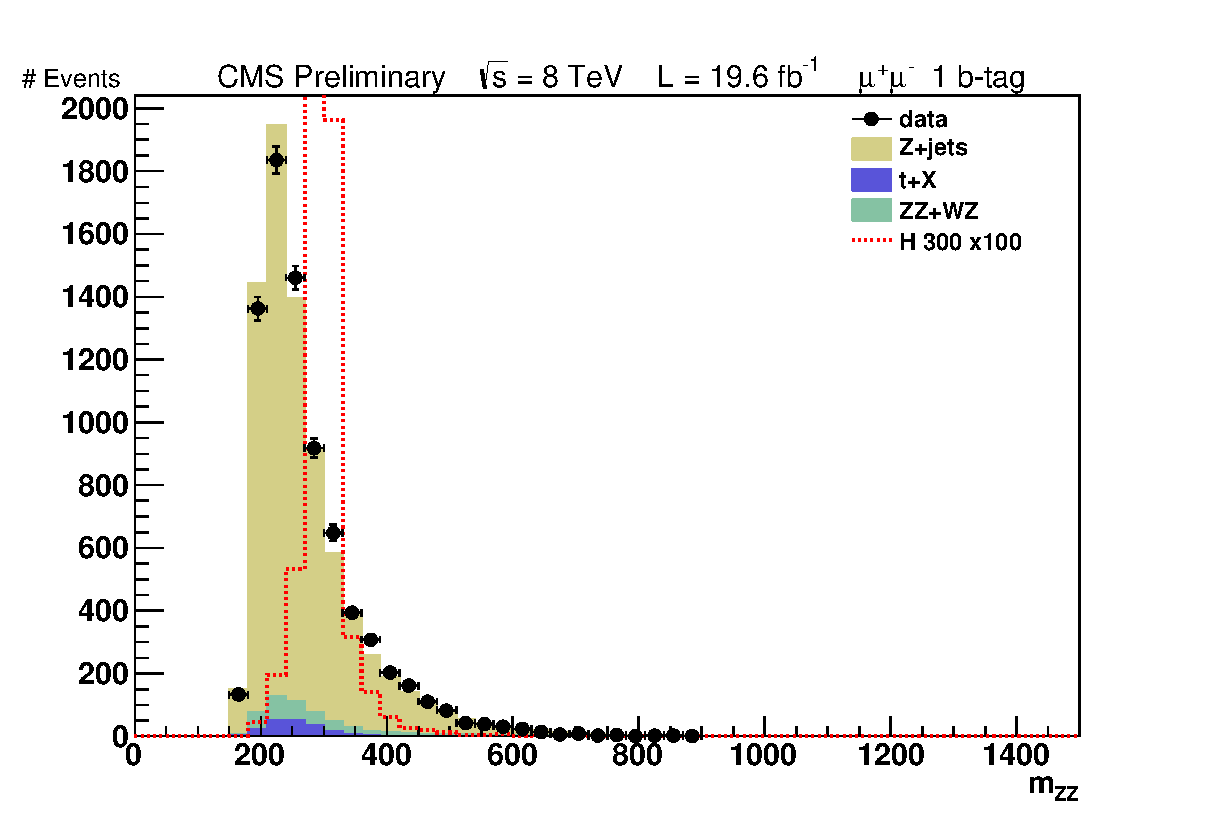
\includegraphics[width=0.33\textwidth]{presentation/defense/images/final/1/mu/mZZ_signal.eps}
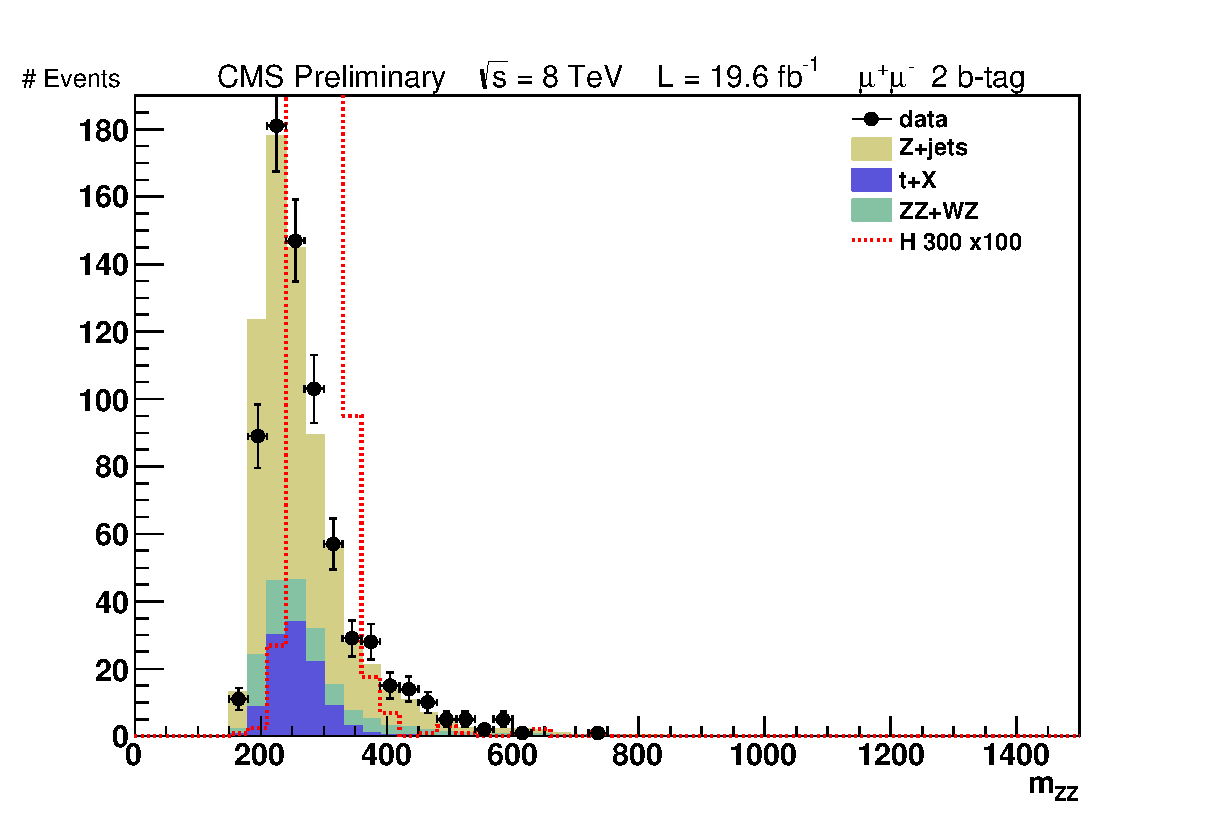
\includegraphics[width=0.33\textwidth]{presentation/defense/images/final/2/mu/mZZ_signal.eps}
}
\caption{Mass distributions of the $\LL jj$ system for events in the signal region in the electron (top) and muon (bottom) channels. From left to right, plots correspond to the 0-, 1-, and 2-btag categories.}
\label{fig:ichepllqq}
\end{center}
\end{figure}
%%%%%%%%%%%%%%%%%%%%%%%%%%%%%%%%%%%%%%%%%%%%%
\begin{figure}[htb]
\begin{center}
\centerline{
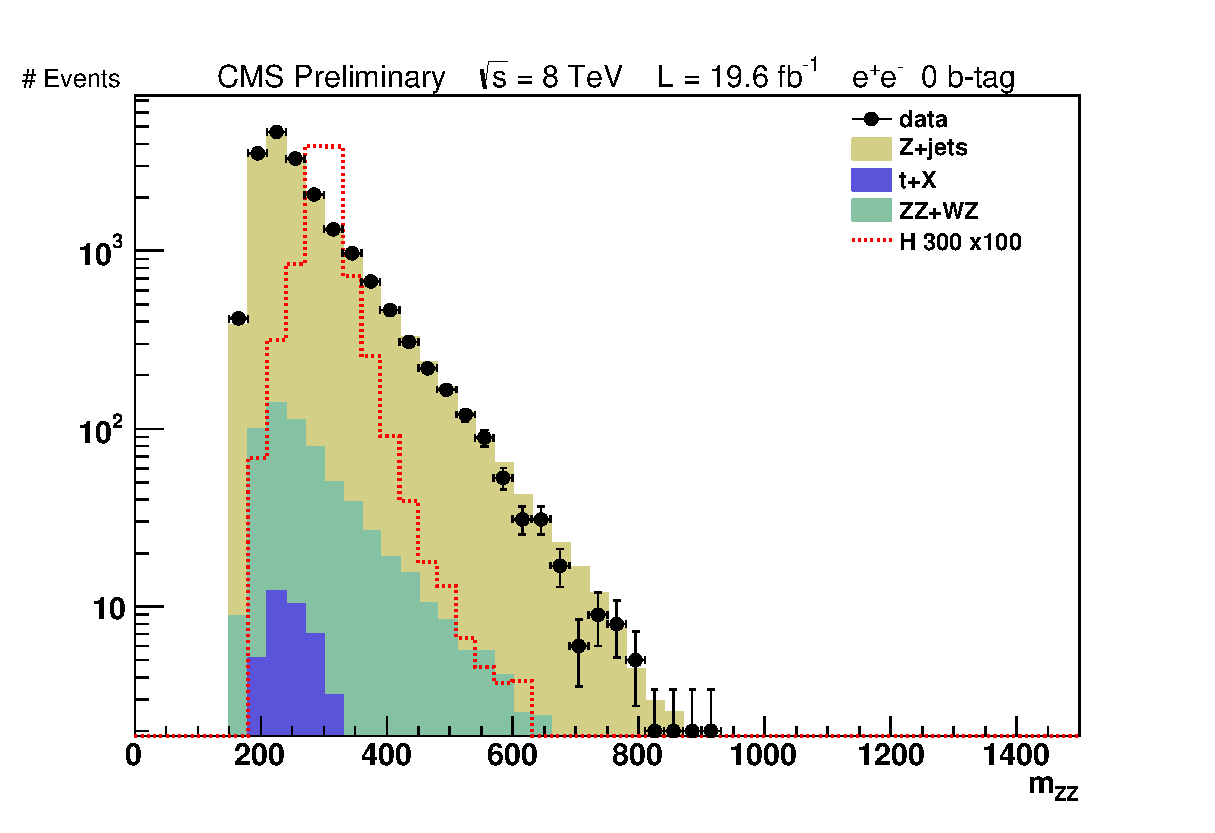
\includegraphics[width=0.33\textwidth]{presentation/defense/images/final/0/el/mZZ_signal_log.eps}
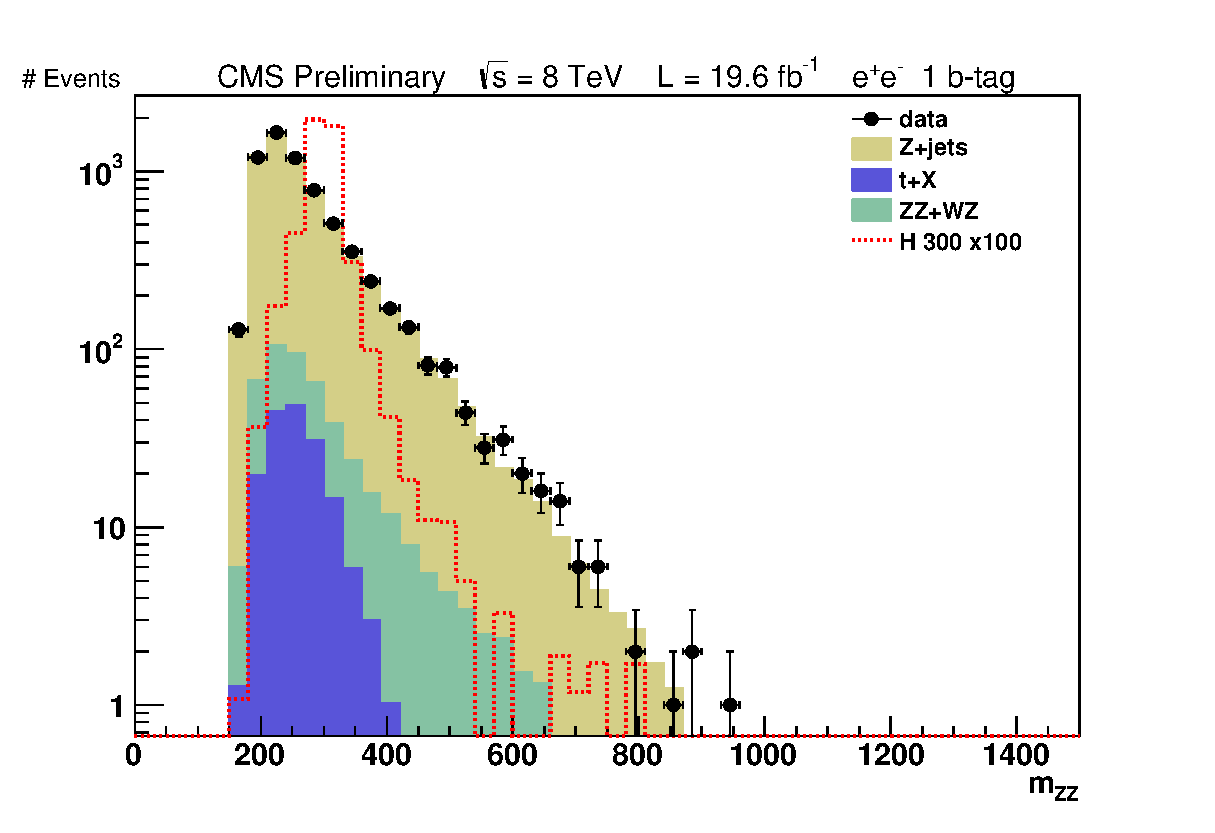
\includegraphics[width=0.33\textwidth]{presentation/defense/images/final/1/el/mZZ_signal_log.eps}
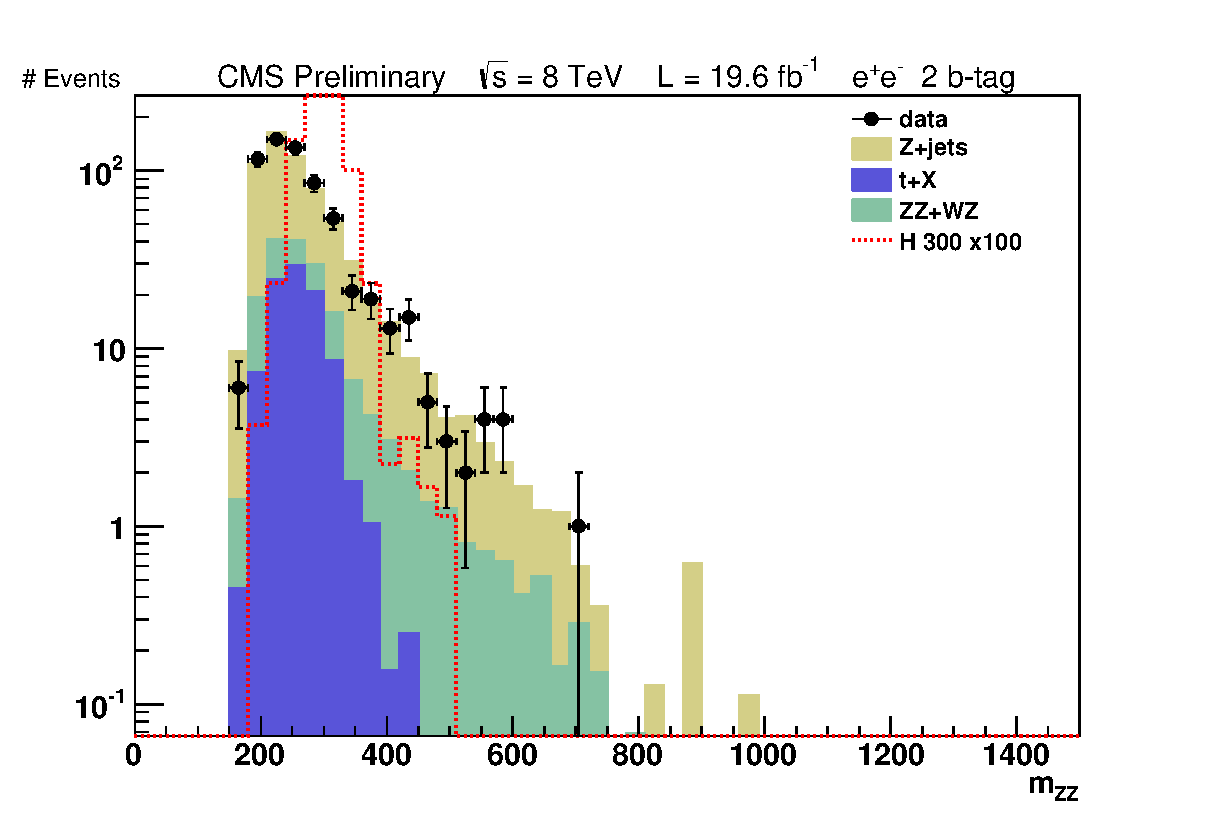
\includegraphics[width=0.33\textwidth]{presentation/defense/images/final/2/el/mZZ_signal_log.eps}
}
\centerline{
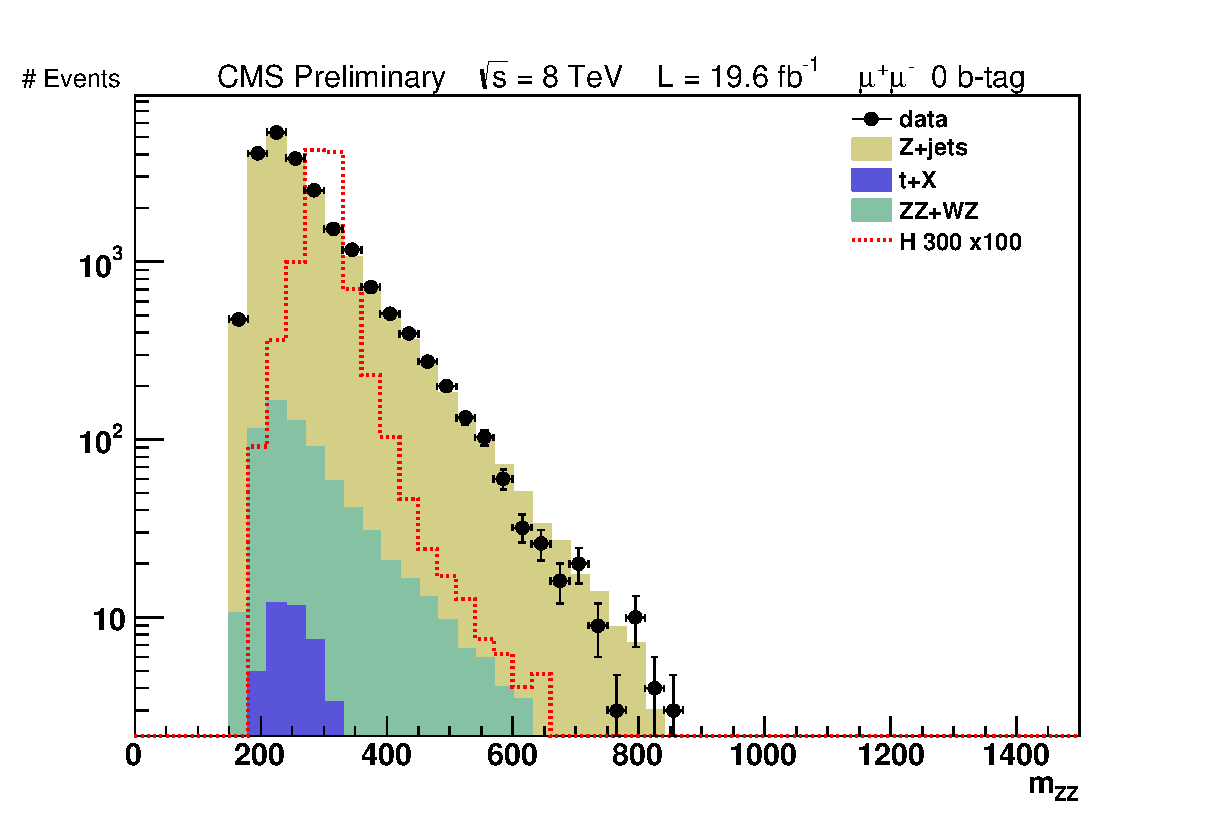
\includegraphics[width=0.33\textwidth]{presentation/defense/images/final/0/mu/mZZ_signal_log.eps}
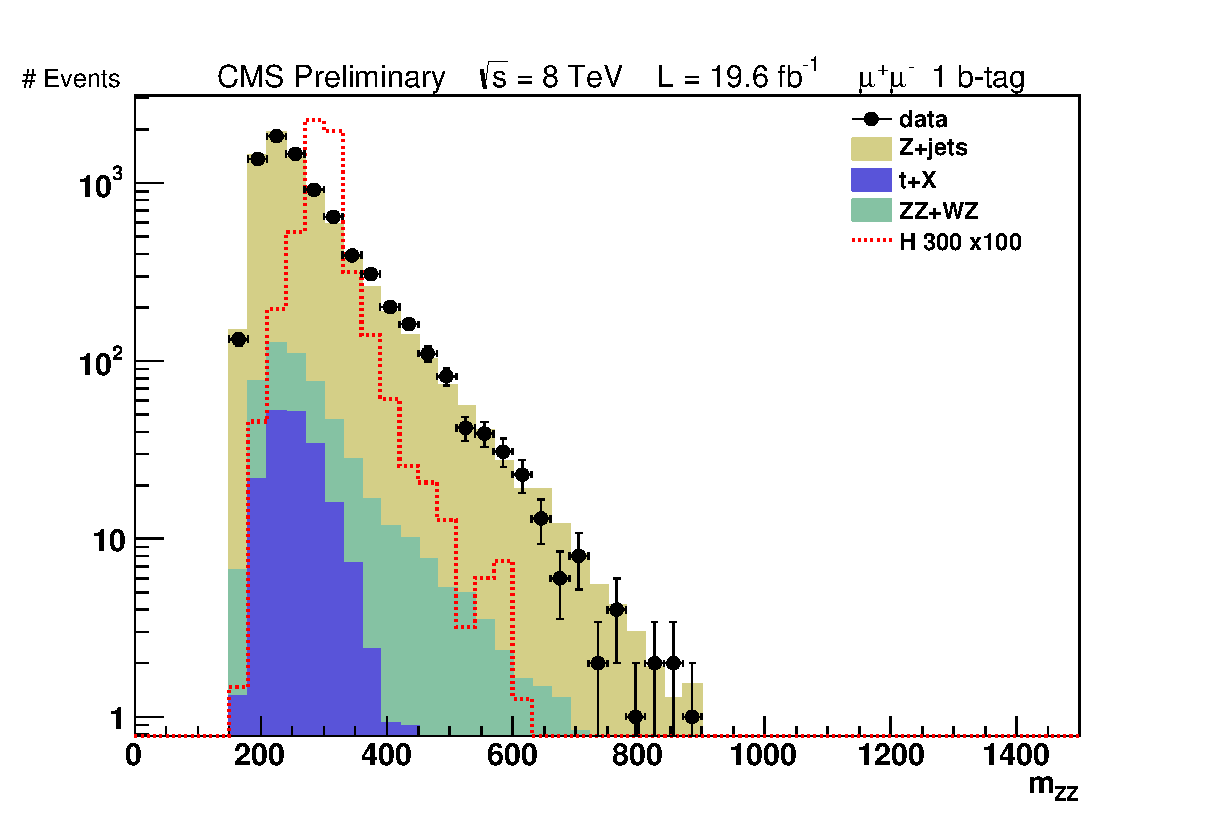
\includegraphics[width=0.33\textwidth]{presentation/defense/images/final/1/mu/mZZ_signal_log.eps}
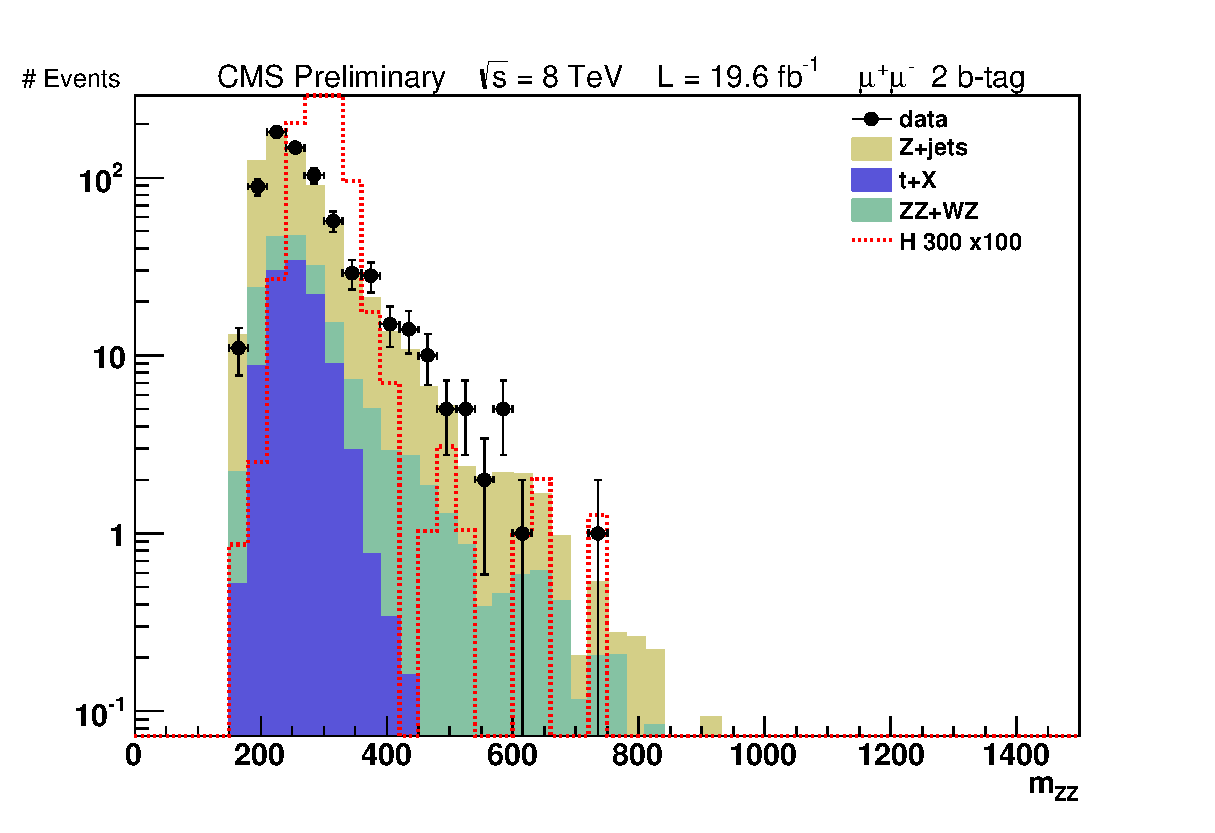
\includegraphics[width=0.33\textwidth]{presentation/defense/images/final/2/mu/mZZ_signal_log.eps}
}
\caption{Mass distributions of Figure~\ref{fig:ichepllqq} in logarithmic scale.
}
\label{fig:ichepllqqLOG}
\end{center}
\end{figure}
%%%%%%%%%%%%%%%%%%%%%%%%%%%%%%%%%%%%%%%%%%%%%
\begin{figure}[htb]
\begin{center}
\centerline{
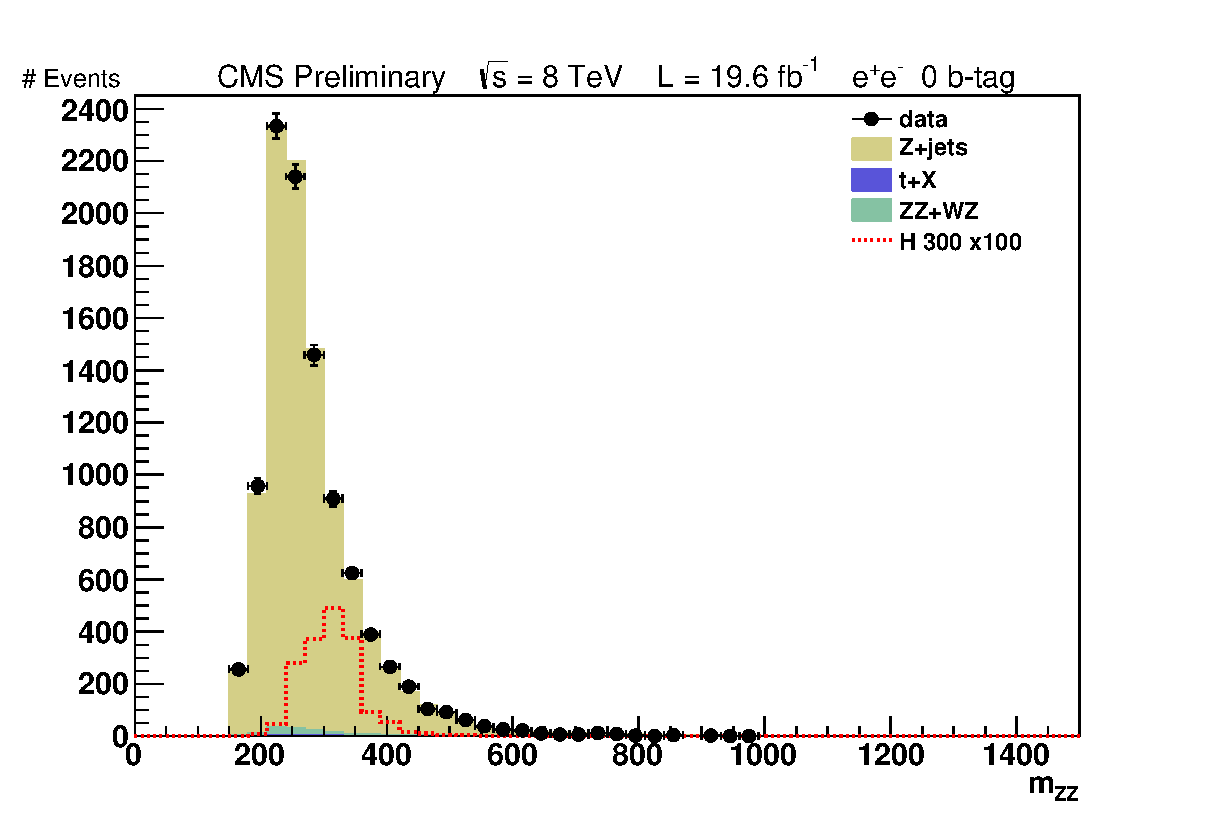
\includegraphics[width=0.33\textwidth]{presentation/defense/images/final/0/el/mZZ_sideband.eps}
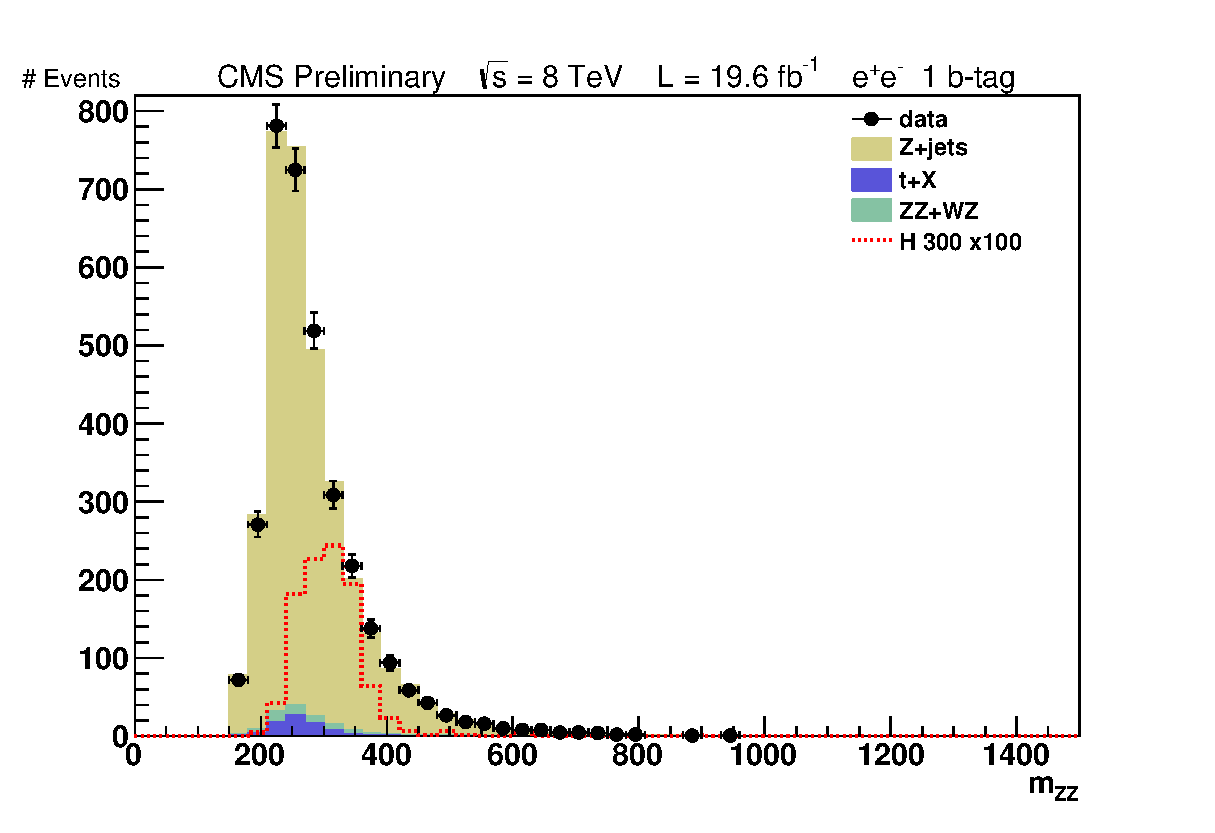
\includegraphics[width=0.33\textwidth]{presentation/defense/images/final/1/el/mZZ_sideband.eps}
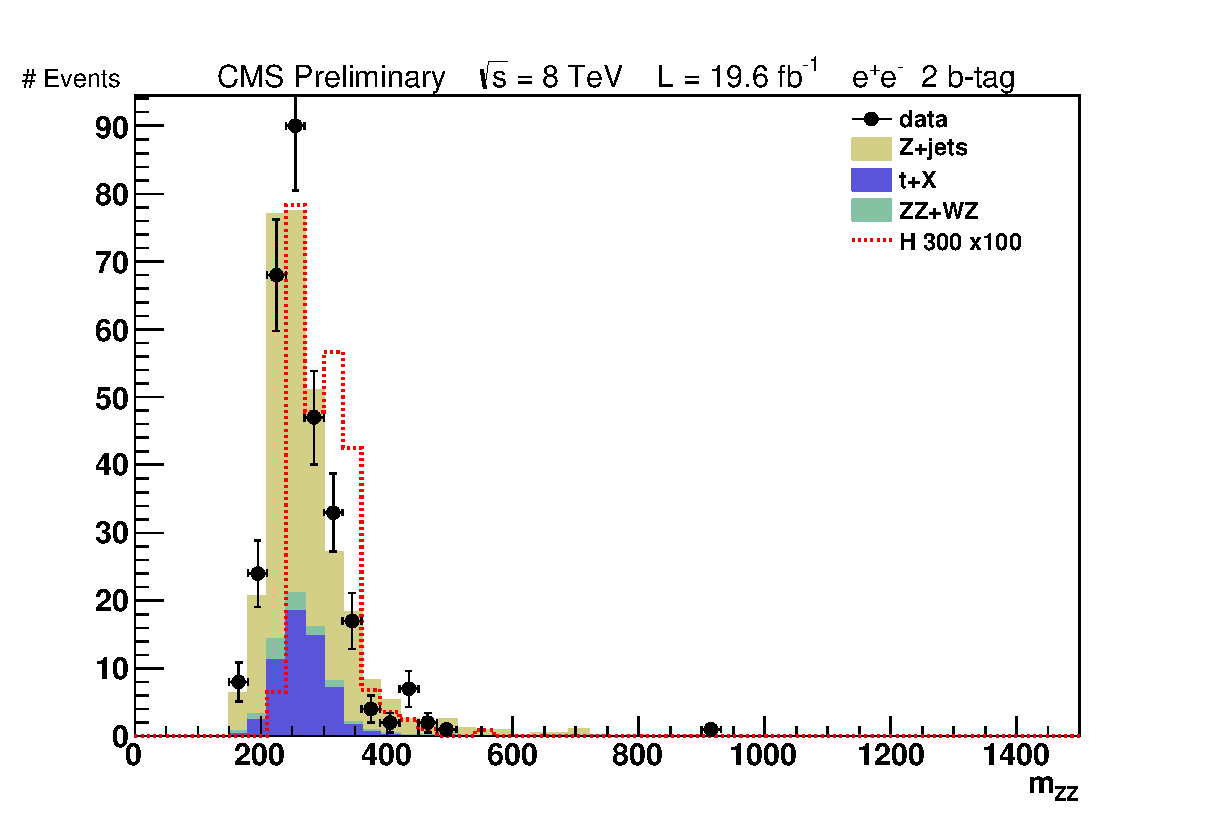
\includegraphics[width=0.33\textwidth]{presentation/defense/images/final/2/el/mZZ_sideband.eps}
}
\centerline{
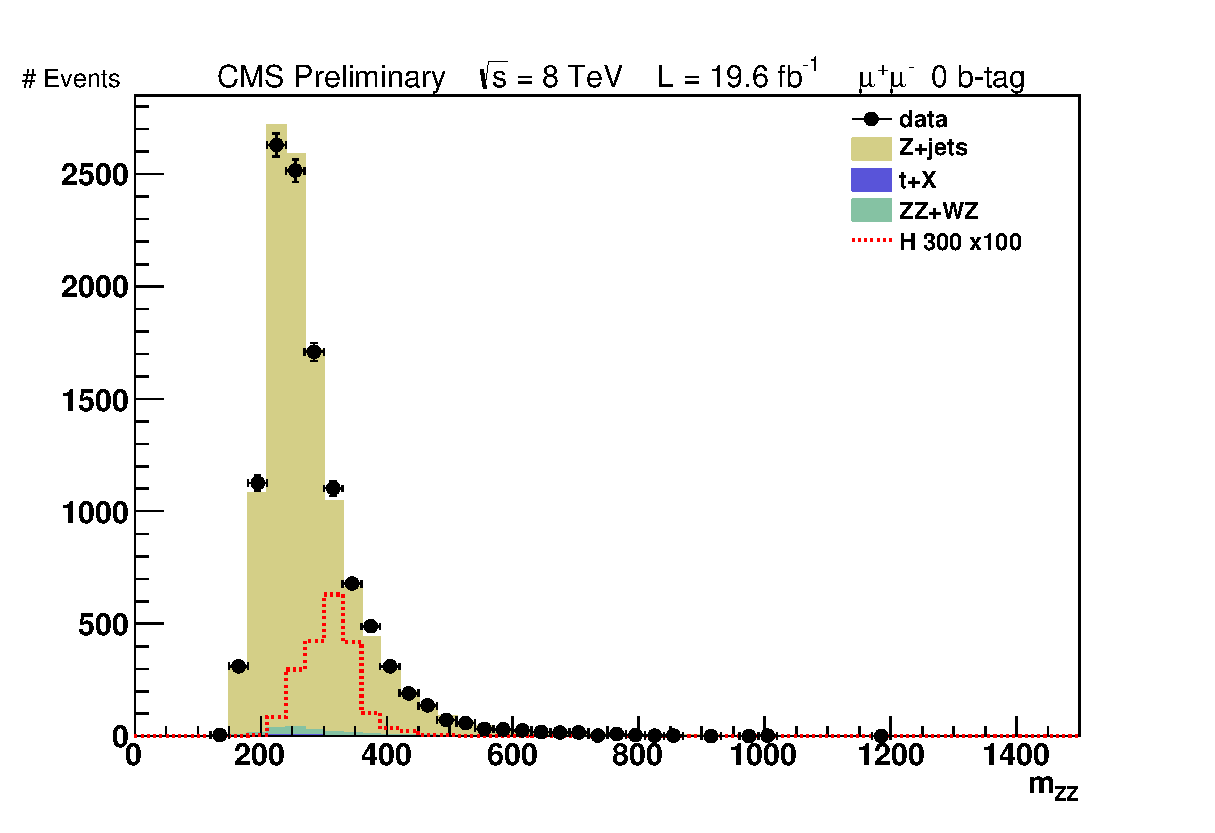
\includegraphics[width=0.33\textwidth]{presentation/defense/images/final/0/mu/mZZ_sideband.eps}
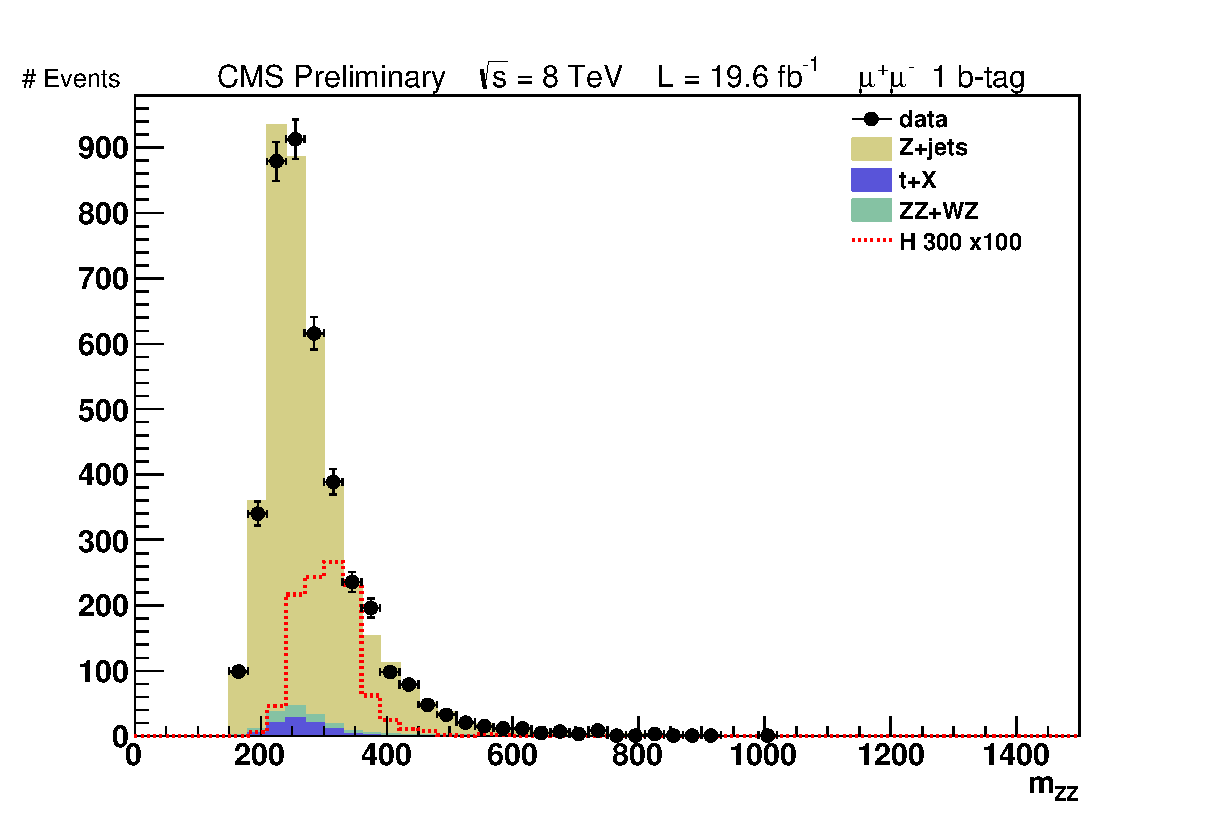
\includegraphics[width=0.33\textwidth]{presentation/defense/images/final/1/mu/mZZ_sideband.eps}
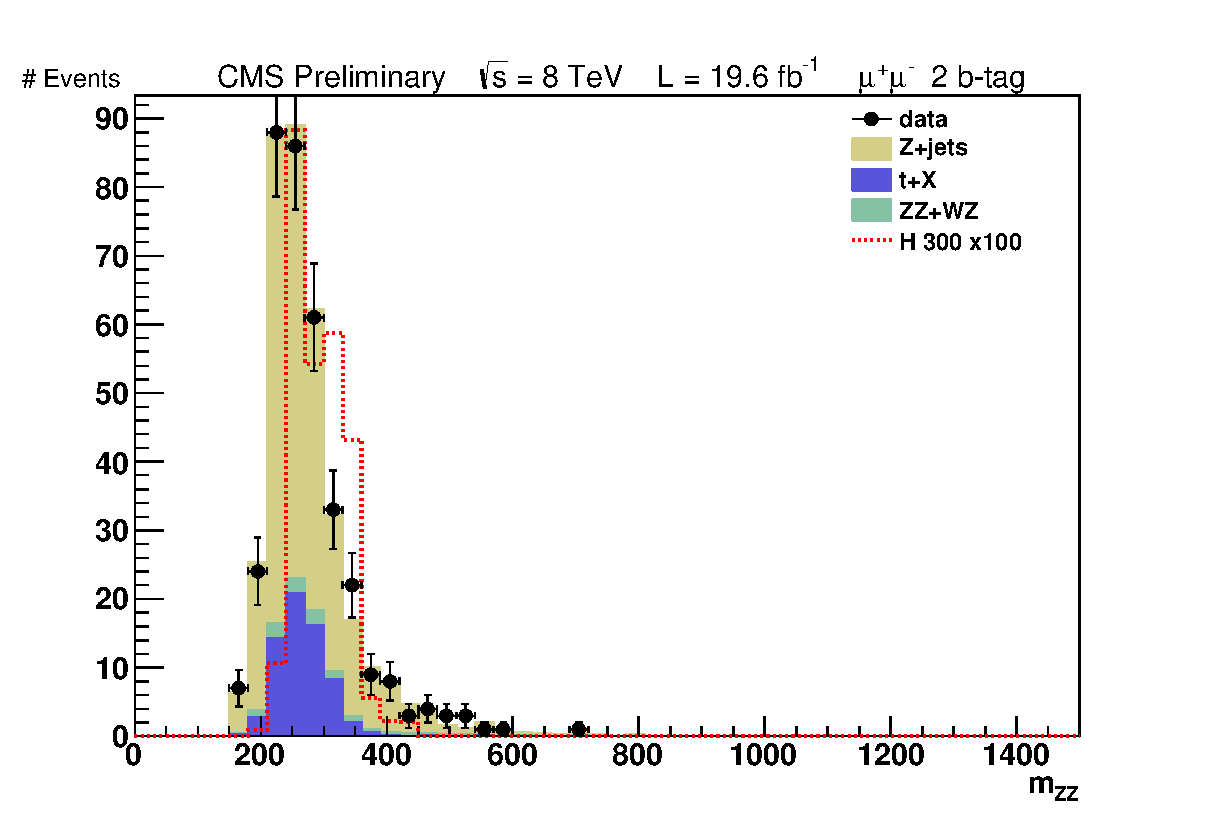
\includegraphics[width=0.33\textwidth]{presentation/defense/images/final/2/mu/mZZ_sideband.eps}
}
\caption{Mass distributions of the $\LL jj$ system for events in the $m_{jj}$ sideband region in the electron (top) and muon (bottom) channels. From left to right, plots correspond to the 0-, 1-, and 2-btag categories.}
\label{fig:llqqSB}
\end{center}
\end{figure}
%%%%%%%%%%%%%%%%%%%%%%%%%%%%%%%%%%%%
\begin{figure}[htb]
\begin{center}
\centerline{
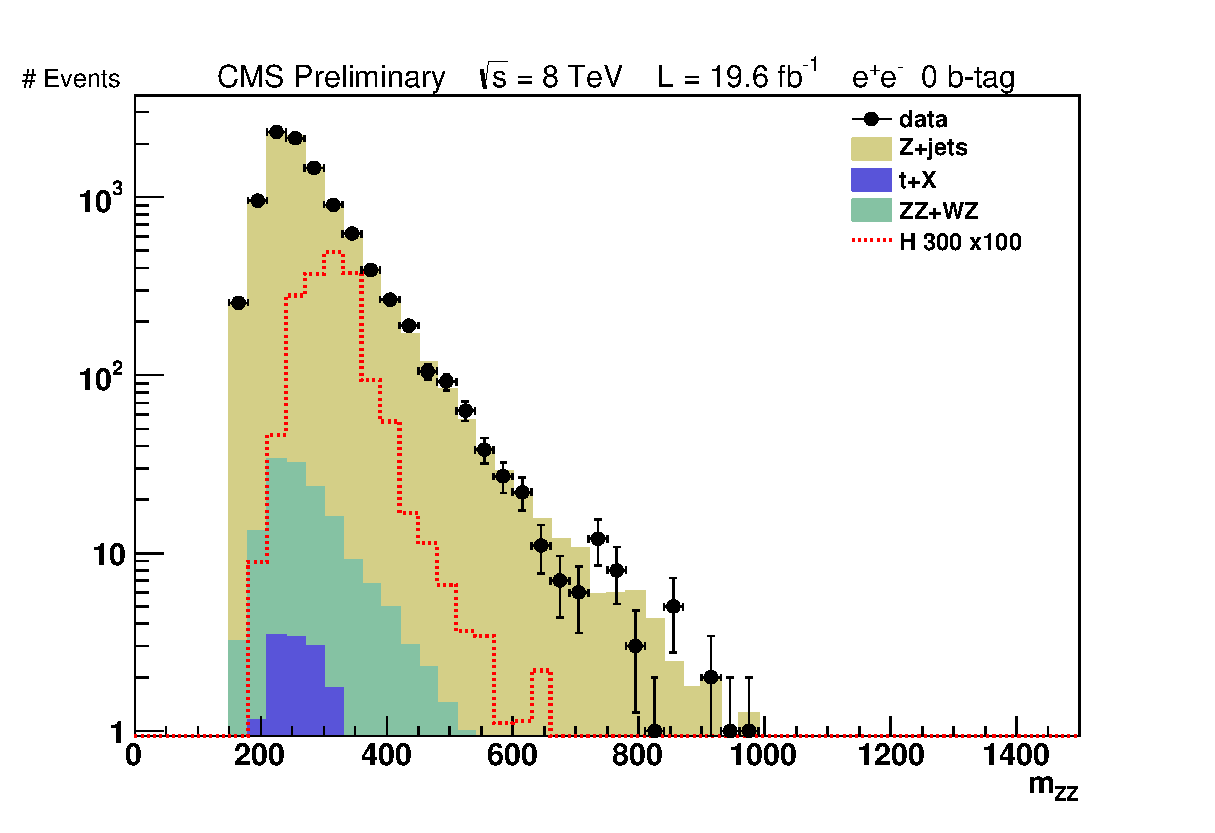
\includegraphics[width=0.33\textwidth]{presentation/defense/images/final/0/el/mZZ_sideband_log.eps}
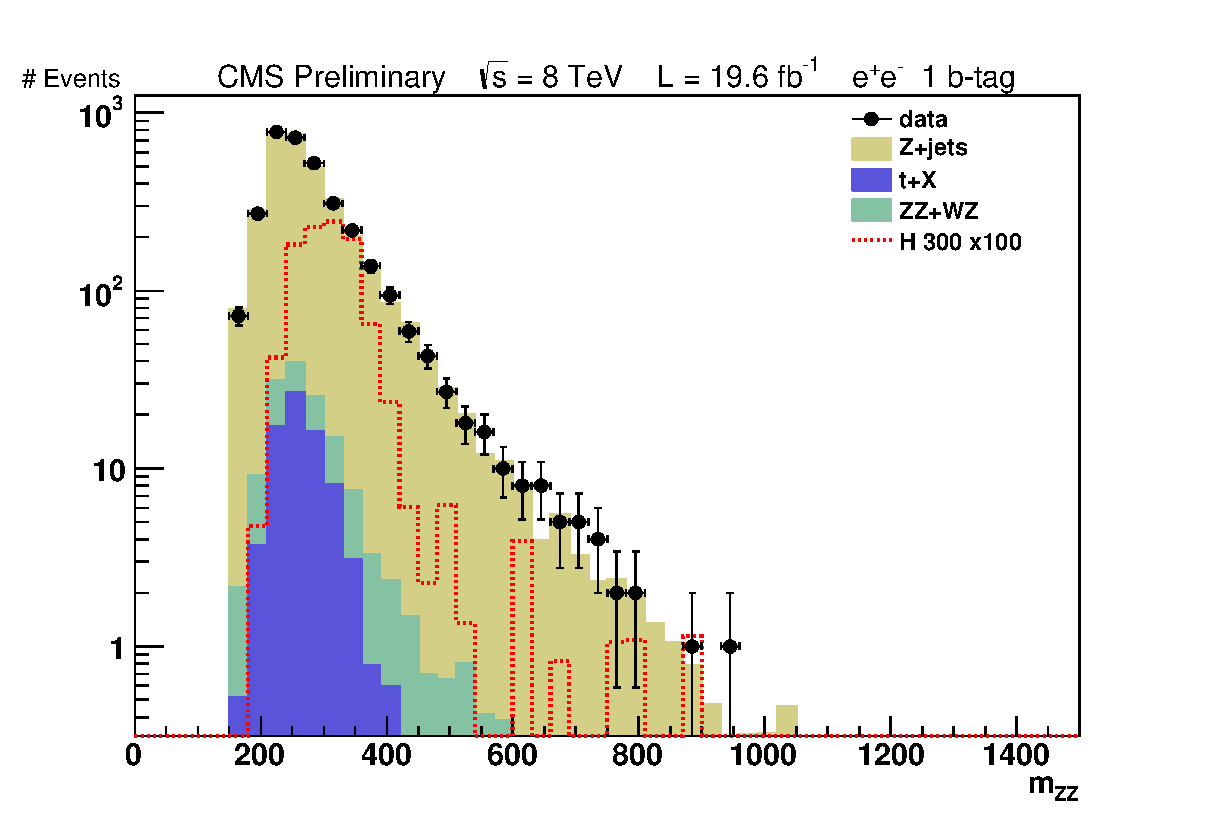
\includegraphics[width=0.33\textwidth]{presentation/defense/images/final/1/el/mZZ_sideband_log.eps}
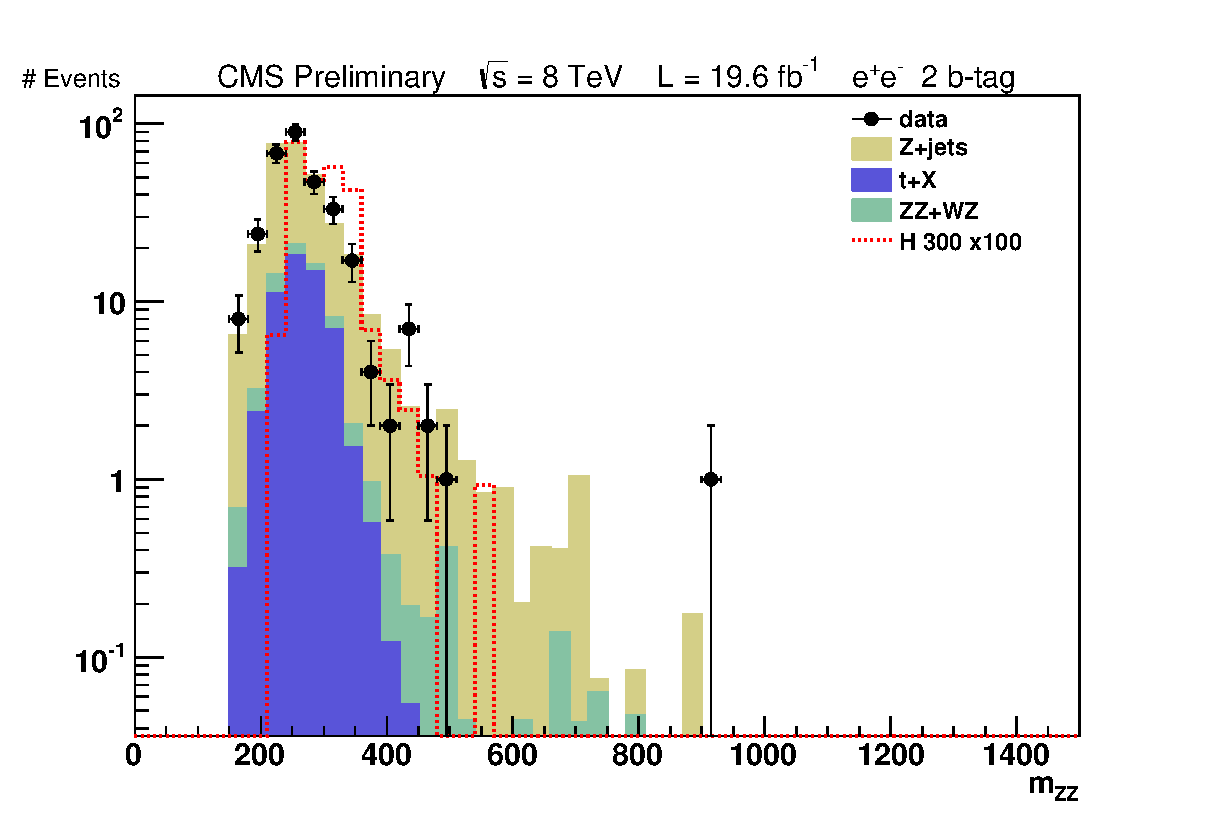
\includegraphics[width=0.33\textwidth]{presentation/defense/images/final/2/el/mZZ_sideband_log.eps}
}
\centerline{
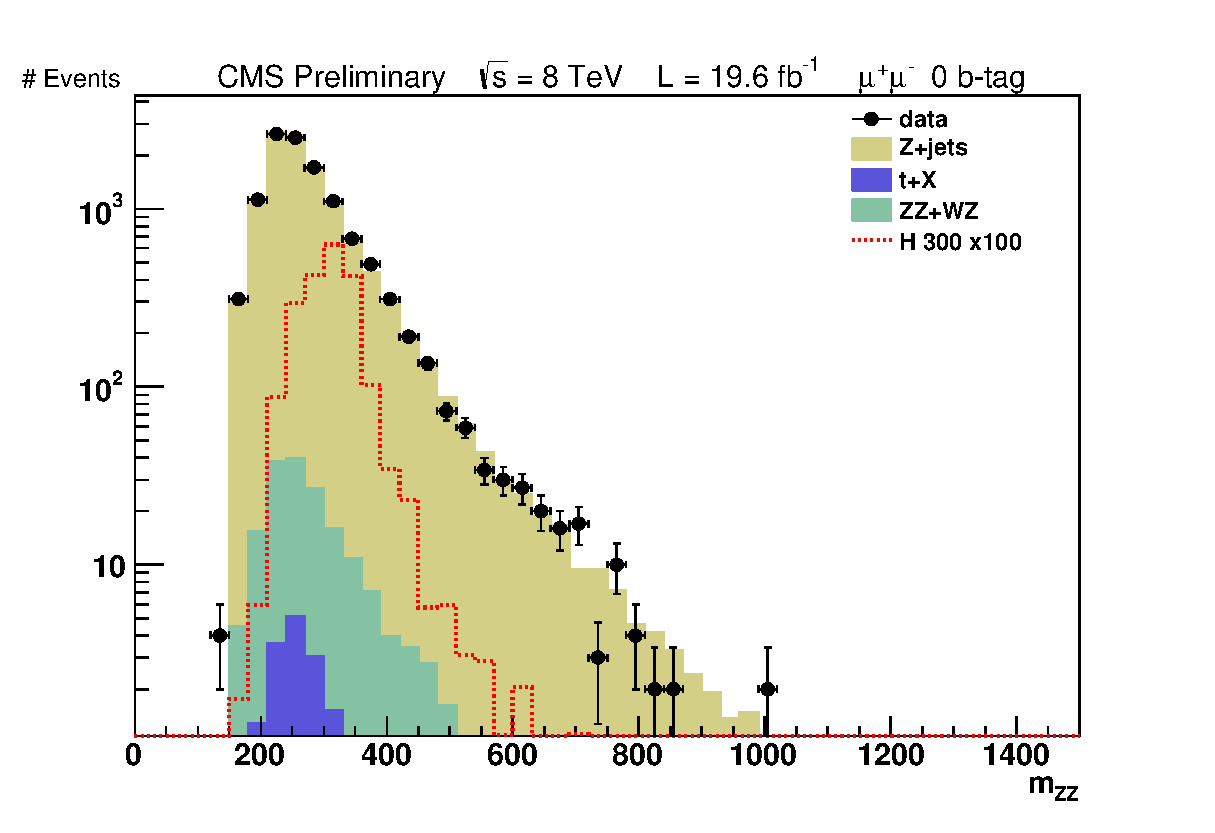
\includegraphics[width=0.33\textwidth]{presentation/defense/images/final/0/mu/mZZ_sideband_log.eps}
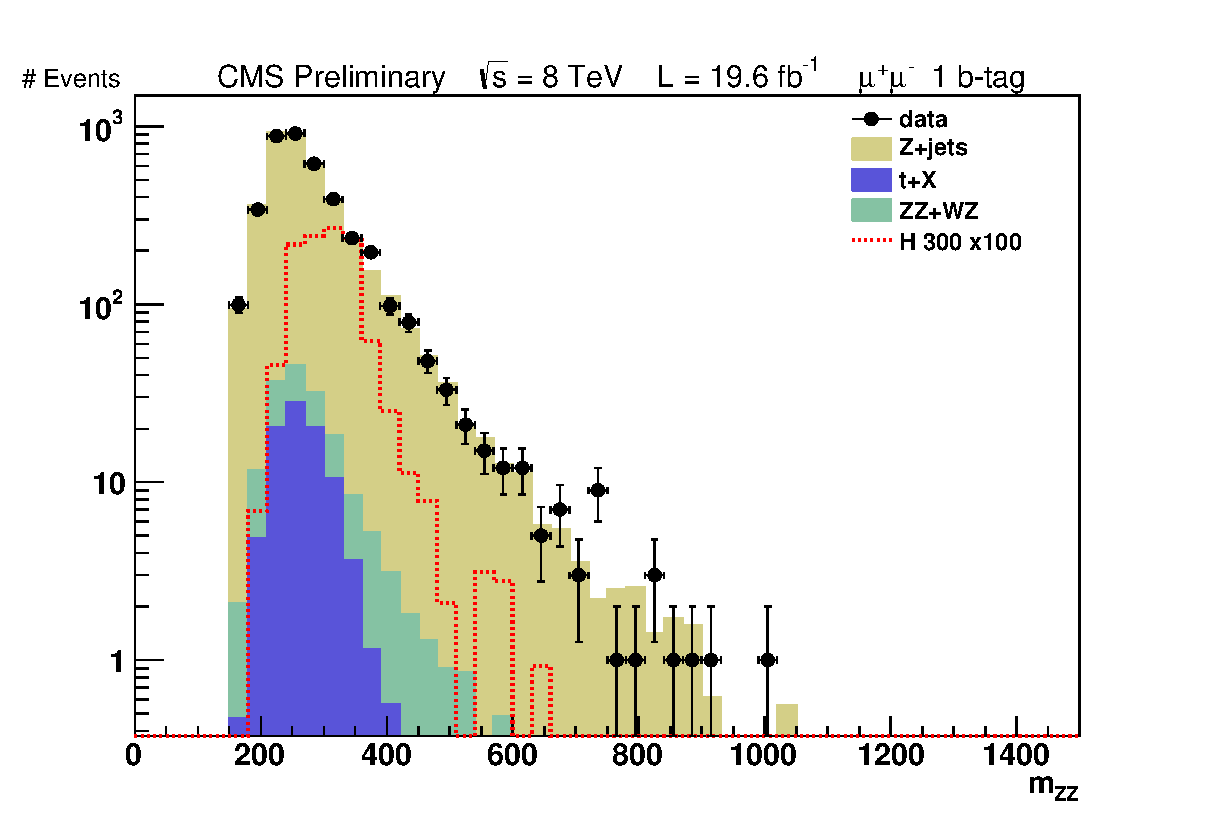
\includegraphics[width=0.33\textwidth]{presentation/defense/images/final/1/mu/mZZ_sideband_log.eps}
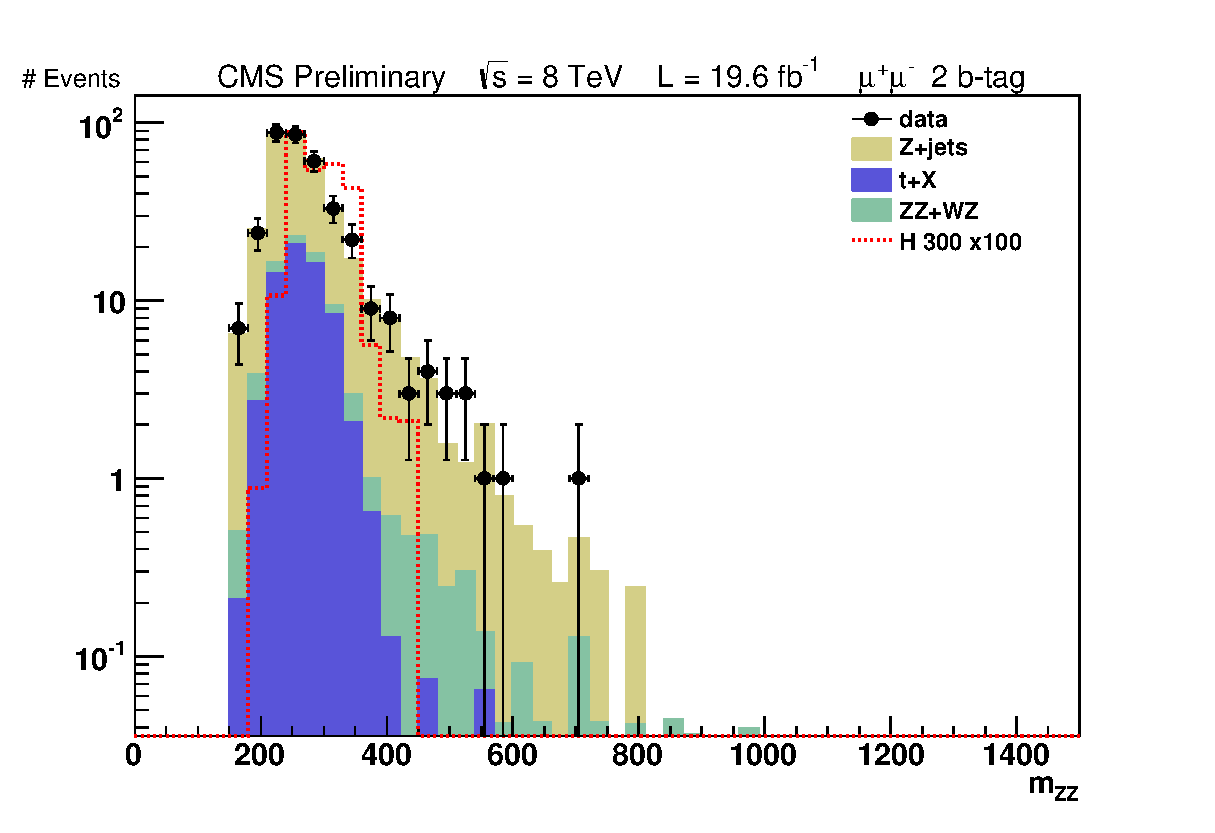
\includegraphics[width=0.33\textwidth]{presentation/defense/images/final/2/mu/mZZ_sideband_log.eps}
}
\caption{Mass distributions of Figure~\ref{fig:llqqSB} in logarithmic scale.}
\label{fig:llqqSBLOG}
\end{center}
\end{figure}
%%%%%%%%%%%%%%%%%%%%%%%%%%%%%%%%%%%%%%%%%%%%%%%%%

Expected upper limits on the SM Higgs boson production cross section are determined as function of the Higgs boson mass hypothesis, taking as input the $\mlljj$ distribution for data, and for the background and signal expectations. The statistical procedure, based on the profile likelihood method, uses the \textit{asymptotic CL$_s$}~\cite{AsymptCLs} approach, implemented in the official tool developed by the CMS Higgs combination group~\cite{HiggsLimitTWiki}. Systematic uncertainties are treated as nuisance parameters.

The results are expressed as upper limits on the ratio of the cross section times branching fraction of the process $\Htollqq\ $, divided by the expectation for the standard model Higgs boson, $\sigma / \sigma_\mathrm{SM}$. A particular Higgs boson mass hypothesis is excluded whenever \mbox{$\sigma / \sigma_\mathrm{SM} < 1$}. The observed limit on $\sigma / \sigma_\mathrm{SM}$ is determined for $\MH$ hypotheses between 230~GeV and 650~GeV, using $\mlljj$ distributions defined in the range from 220~GeV to 800~GeV. The $\mlljj$ region below 220~GeV presents a very sharp rising edge from Z+jets which is difficult to have under control and is excluded from the analysis.

Figure~\ref{fig:limit5fb} shows the expected and observed limits for the full dataset recorded during 2012 at 8~\TeV{}, corresponding to a luminosity of 19.6~\fbinv{}. With the increased luminosity in this dataset the 2-btag category becomes the most powerful contribution to the combination of the six channels (Figure~\ref{fig:limit20fb_split}). These results were cross-checked with an independent statistical method (Appendix~\ref{sec:cutcount}).
%Other CMS searches have produced limits with on a much finer grid of resonance mass hypothesis. In order to combine our results with these searches, we interpolate the histograms used as for the signal hypothesis to those points where no simulation is available. For this interpolation we use the Radial-Basis-Function (RBF) method~\cite{numrec}.

Limits on the SM production cross section times branching fraction for $\HZZ$ are presented in Figure~\ref{fig:limitxs}. For comparison, expectations are shown for a SM-like Higgs boson. In addition, the limits as observed in this study are combined with the results of the previous analysis on the 2011 data sets~\cite{HIG-11-027}, as shown in Figure~\ref{fig:combination}.

% %Limits on the SM product cross section times branching fraction for
% %$H\to ZZ$ are presented in Figure~\ref{fig:plot_ul}.
% According to the result after unblinding, the result of this analysis excludes the existence of a
% resonance with properties as those of the SMHiggs in the mass range between 269~GeV and 304~GeV,
 % and between 360~GeV and 555~GeV, with the first 5~$\fbinv$ of unblinded data.
% The expected sensitivity of the analysis with the full 8~\TeV{} dataset should allow discovery/exclusion
% of a Higgs boson signal in the full mass range considered (230~GeV to 650~GeV).

% \begin{figure}[htbp]
% \begin{center}
% \centerline{
% 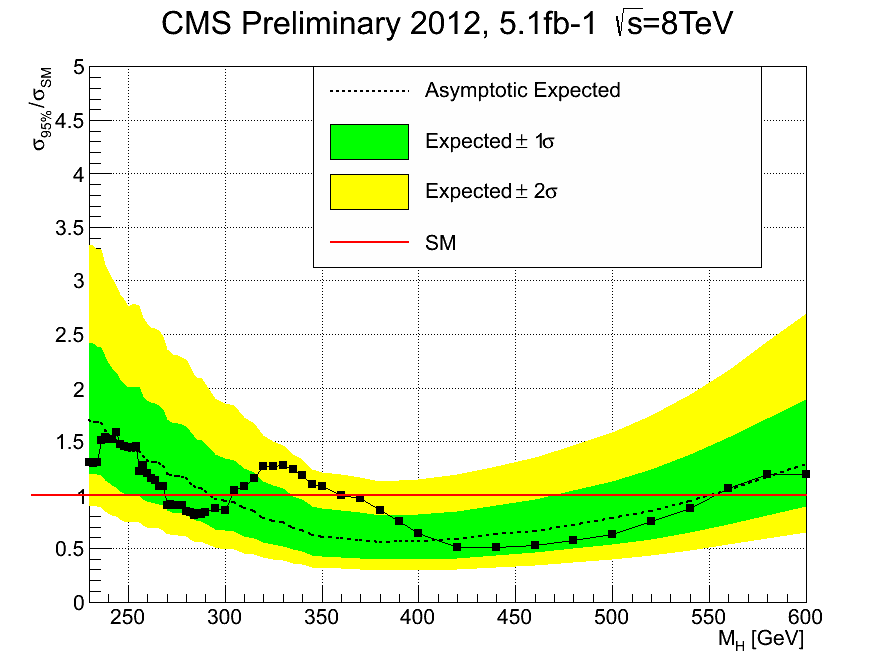
\includegraphics[width=0.49\textwidth]{plots/limit_histo_5fb_unblinded.png}
% 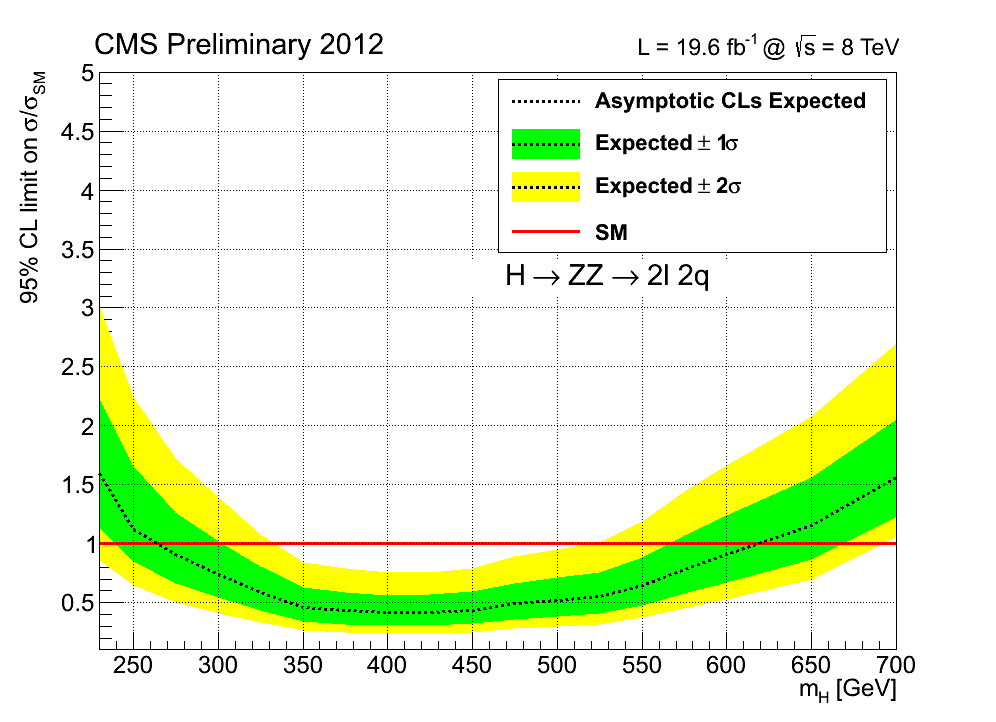
\includegraphics[width=0.49\textwidth]{plots/limit_histo_20fb_blinded.png}
% }
% \centerline{
% 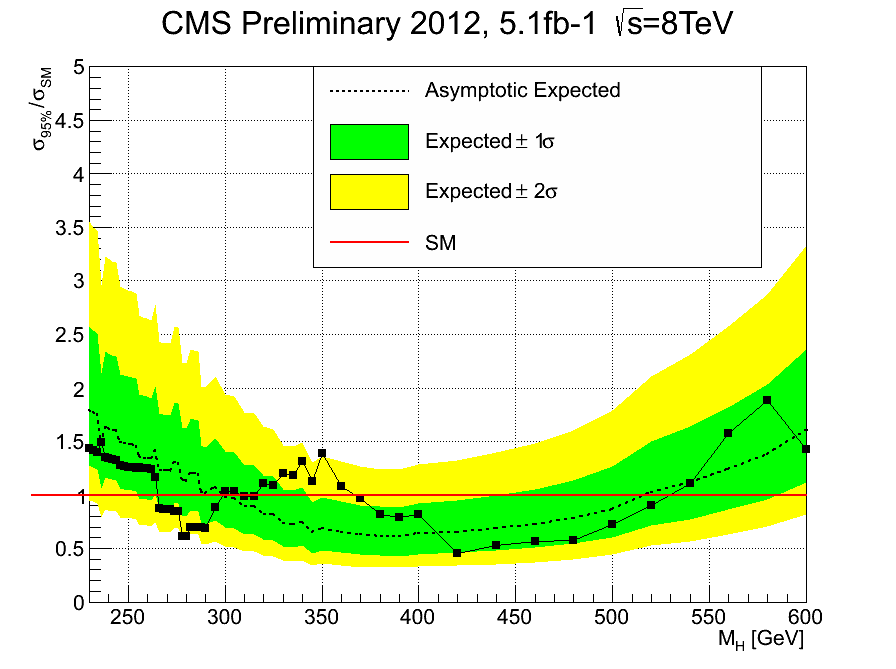
\includegraphics[width=0.49\textwidth]{plots/limit_CiC5_5fb_unblinded.png}
% 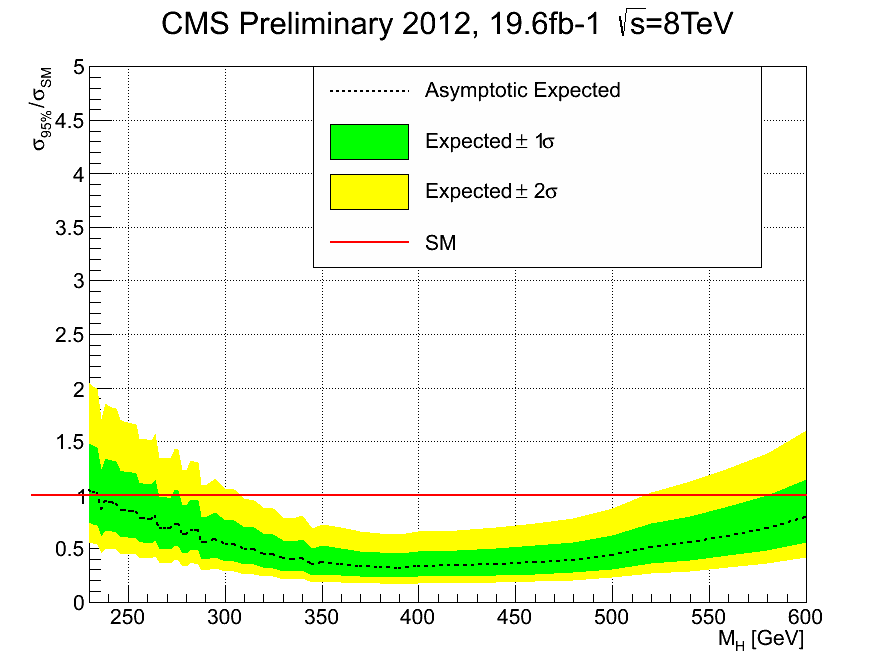
\includegraphics[width=0.49\textwidth]{plots/limit_CiC20_blinded.png}
% }
% \caption{
% Upper limits at the 95$\%$ CL on the Higgs boson production cross section times
% the H$\rightarrow$ZZ branching fraction (upper left) observed and expected using 5.1~\fbinv{} of data,
% and (upper right) expected for 19.6~\fbinv{}. The dots correspond to the observed
% limit and dashed line to the expected one. Yellow and green bands represent the 68$\%$
% and 95$\%$ ranges of expectation.
% The two lower plots, calculated with the cut-and-count method, are displayed as a mere cross check. 
% }
% \label{fig:limit5fb}
% \end{center}
% \end{figure}

\begin{figure}[htbp]
\centerline{
% 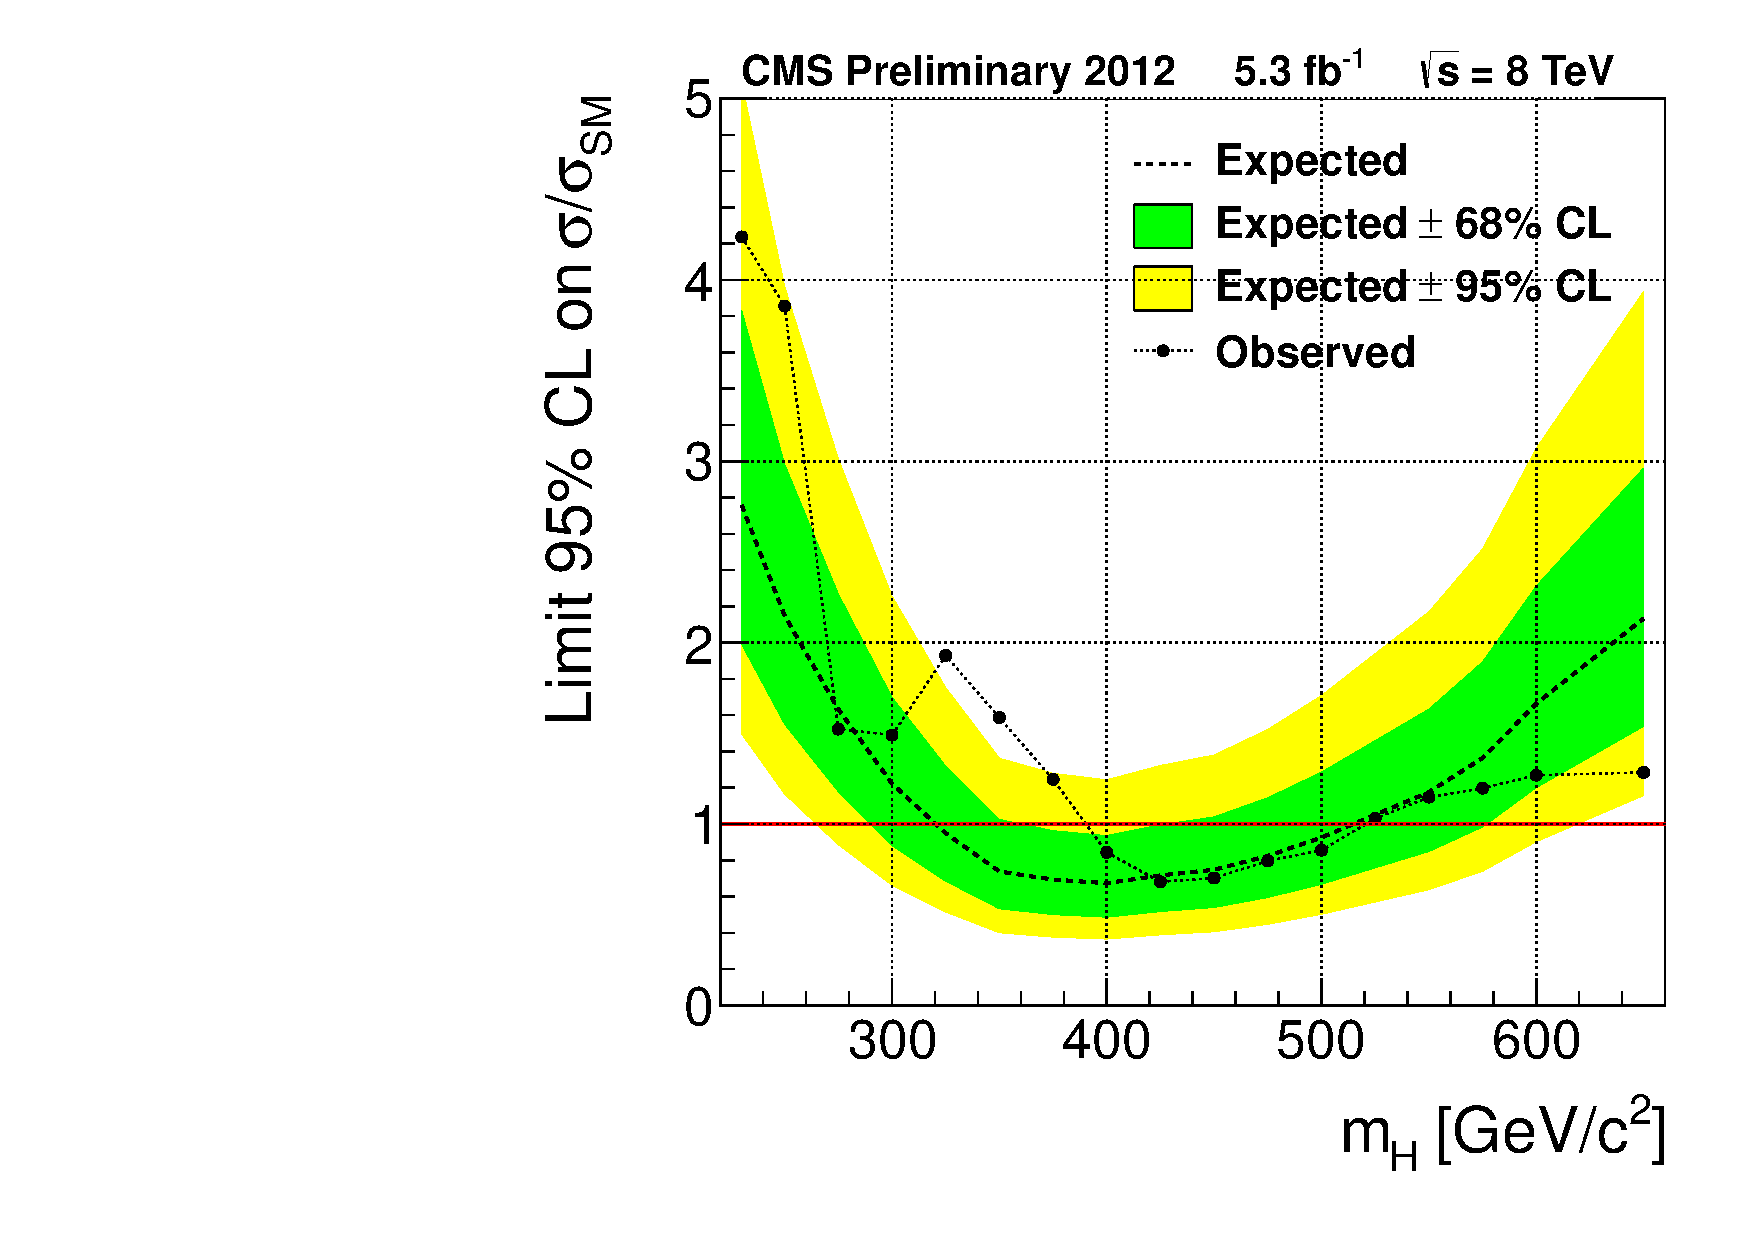
\includegraphics[width=0.49\textwidth]{plots/limit_observed_ICHEP.pdf}
 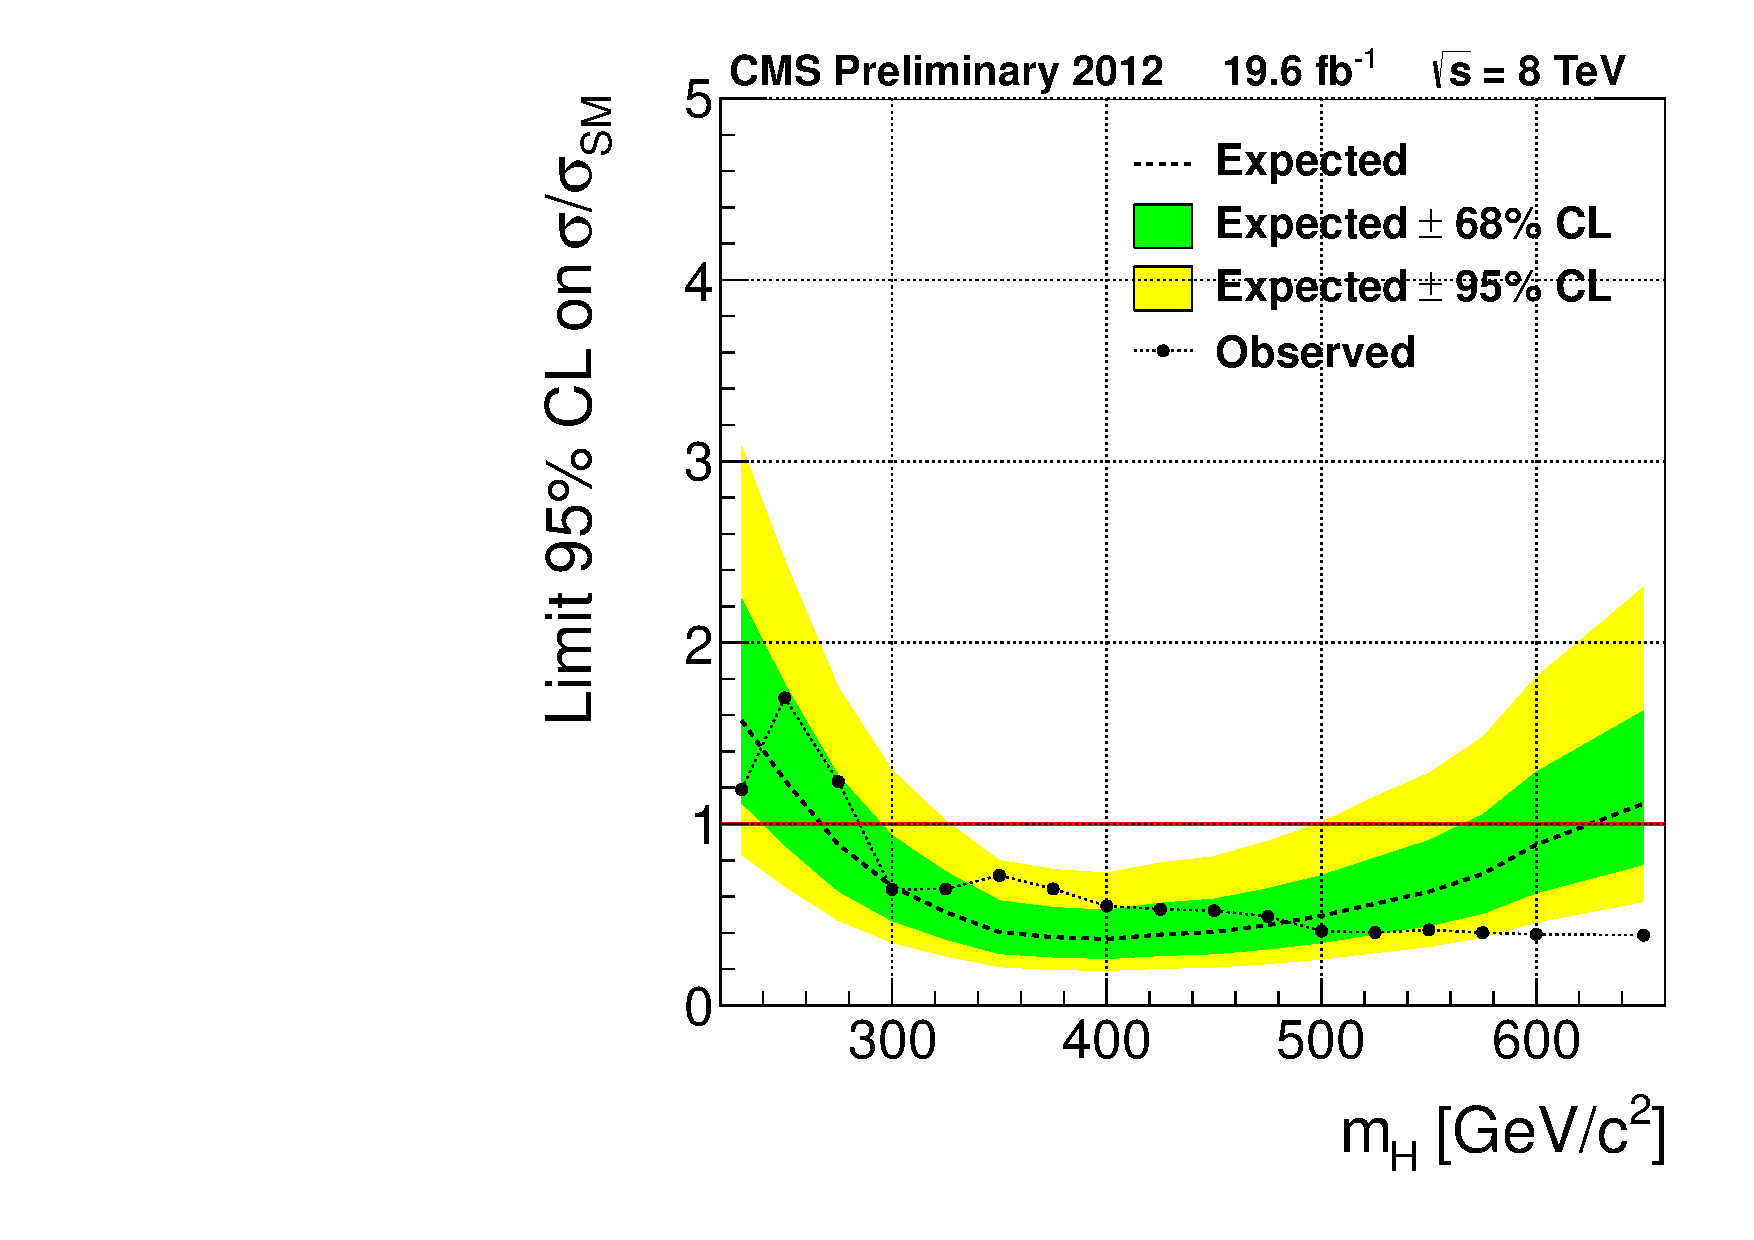
\includegraphics[width=0.79\textwidth]{plots/limit_observed_all-btag_ll.pdf}
%}
% \centerline{
% 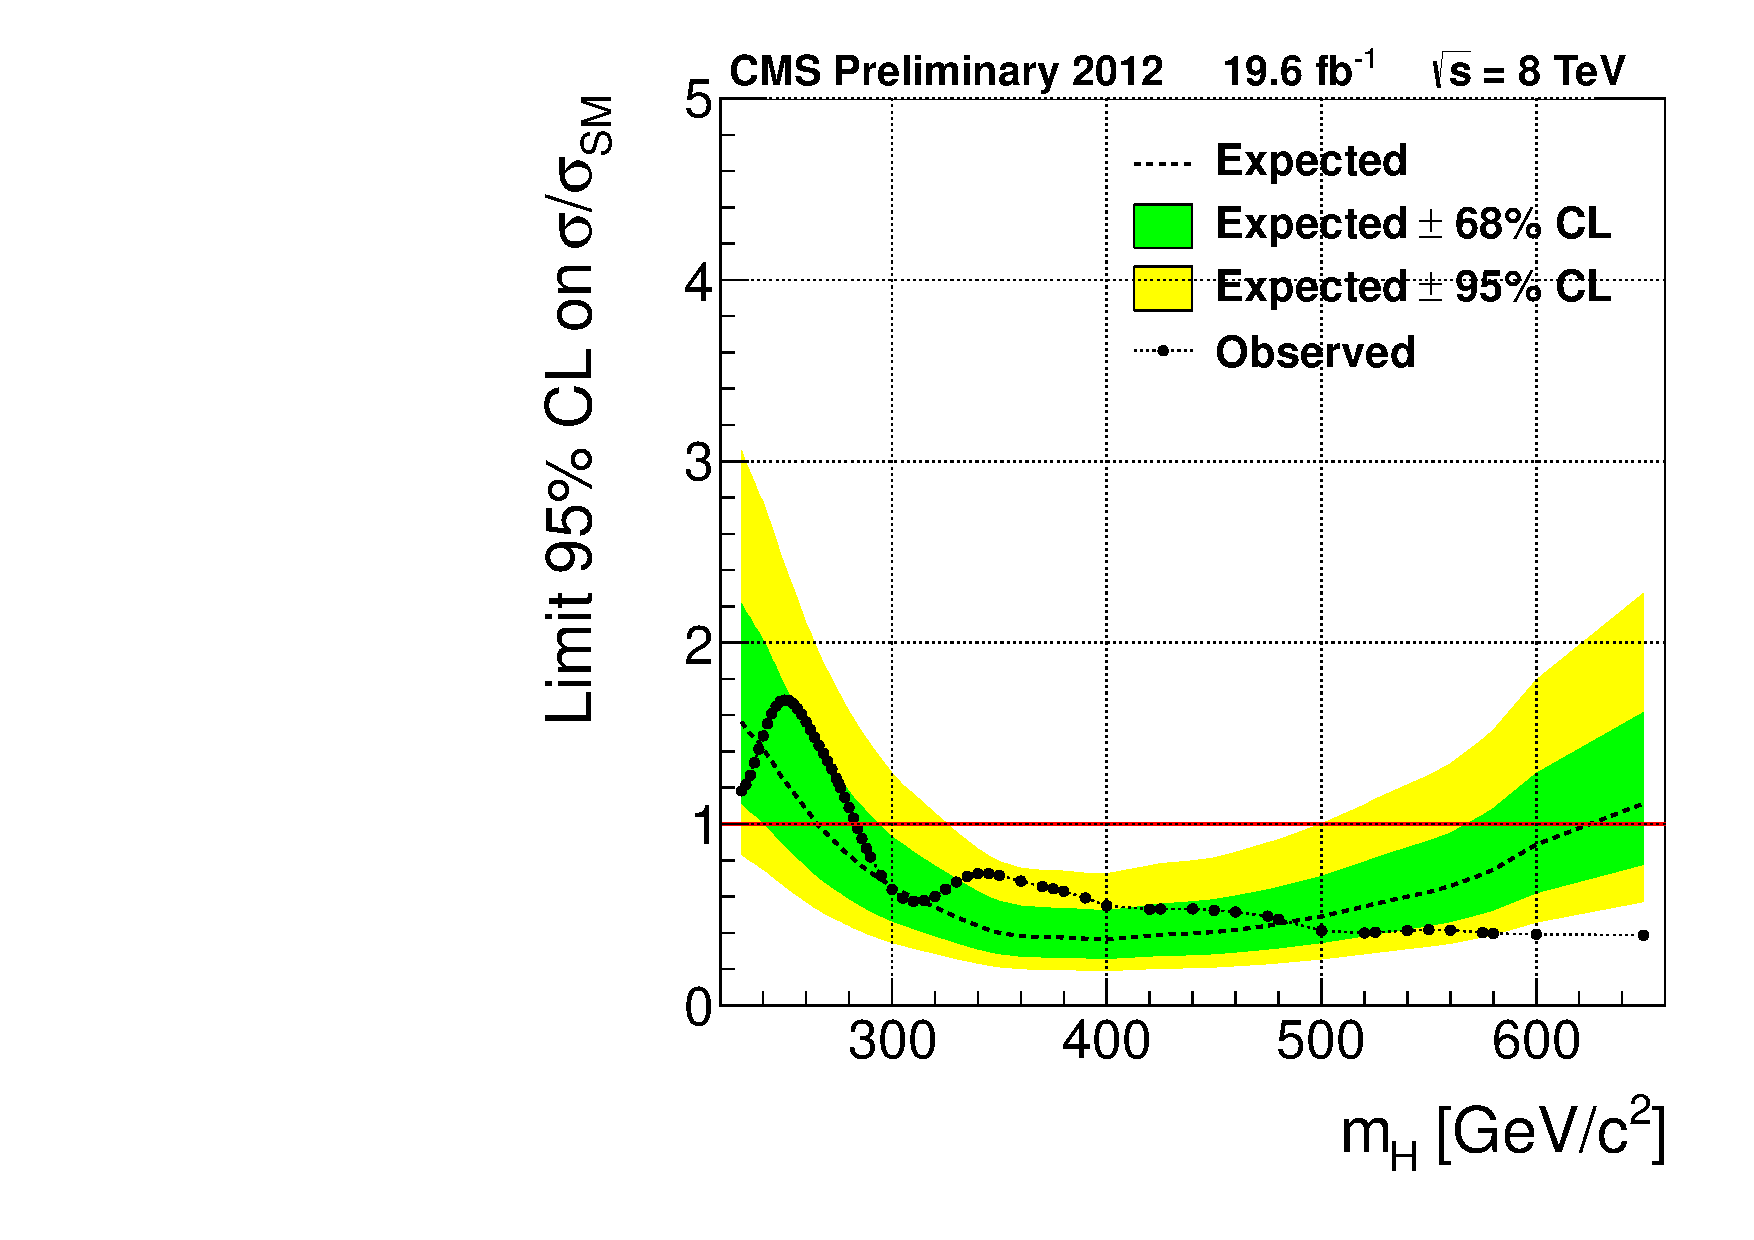
\includegraphics[width=0.49\textwidth]{plots/limit_observed_all-btag_ll_interpol.pdf}
}
\caption{
%Observed (solid) and expected (dashed) 95\% CL upper limit on the ratio of the production cross section to the SM expectation for the Higgs boson obtained using the $\mathrm{CL_s}$ technique. The 68\% and 95\% ranges of expectation for the background-only model are also shown with green and yellow bands, respectively.  The solid line at 1 indicates the expectation for a SM-Higgs-like boson. The results on the top left correspond to a check performed on the unblinded part of the dataset (ICHEP data) to verify everything is under control. The plot on the top right shows the expected and observed limits using 19.6~\fbinv{} of data. The top plots show the observed limit only at the points where the signal shape can be directly obtained from the simulation. The bottom is equivalent to the top right plot, but additionally shows observed limit points where the signal shape has been obtained from interpolation for use in the CMS wide combination of results.
Observed (solid) and expected (dashed) 95\% CL upper limit on the ratio of the production cross section to the SM expectation for the Higgs boson obtained using the $\mathrm{CL_s}$ technique. The 68\% and 95\% ranges of expectation for the background-only model are also shown with green and yellow bands, respectively.  The solid line at 1 indicates the expectation for a SM-Higgs-like boson. The plot shows the expected and observed limits using 19.6~\fbinv{} of data.
}
\label{fig:limit5fb}
\end{figure}

\begin{figure}[htbp]
 \begin{center}
\centerline{
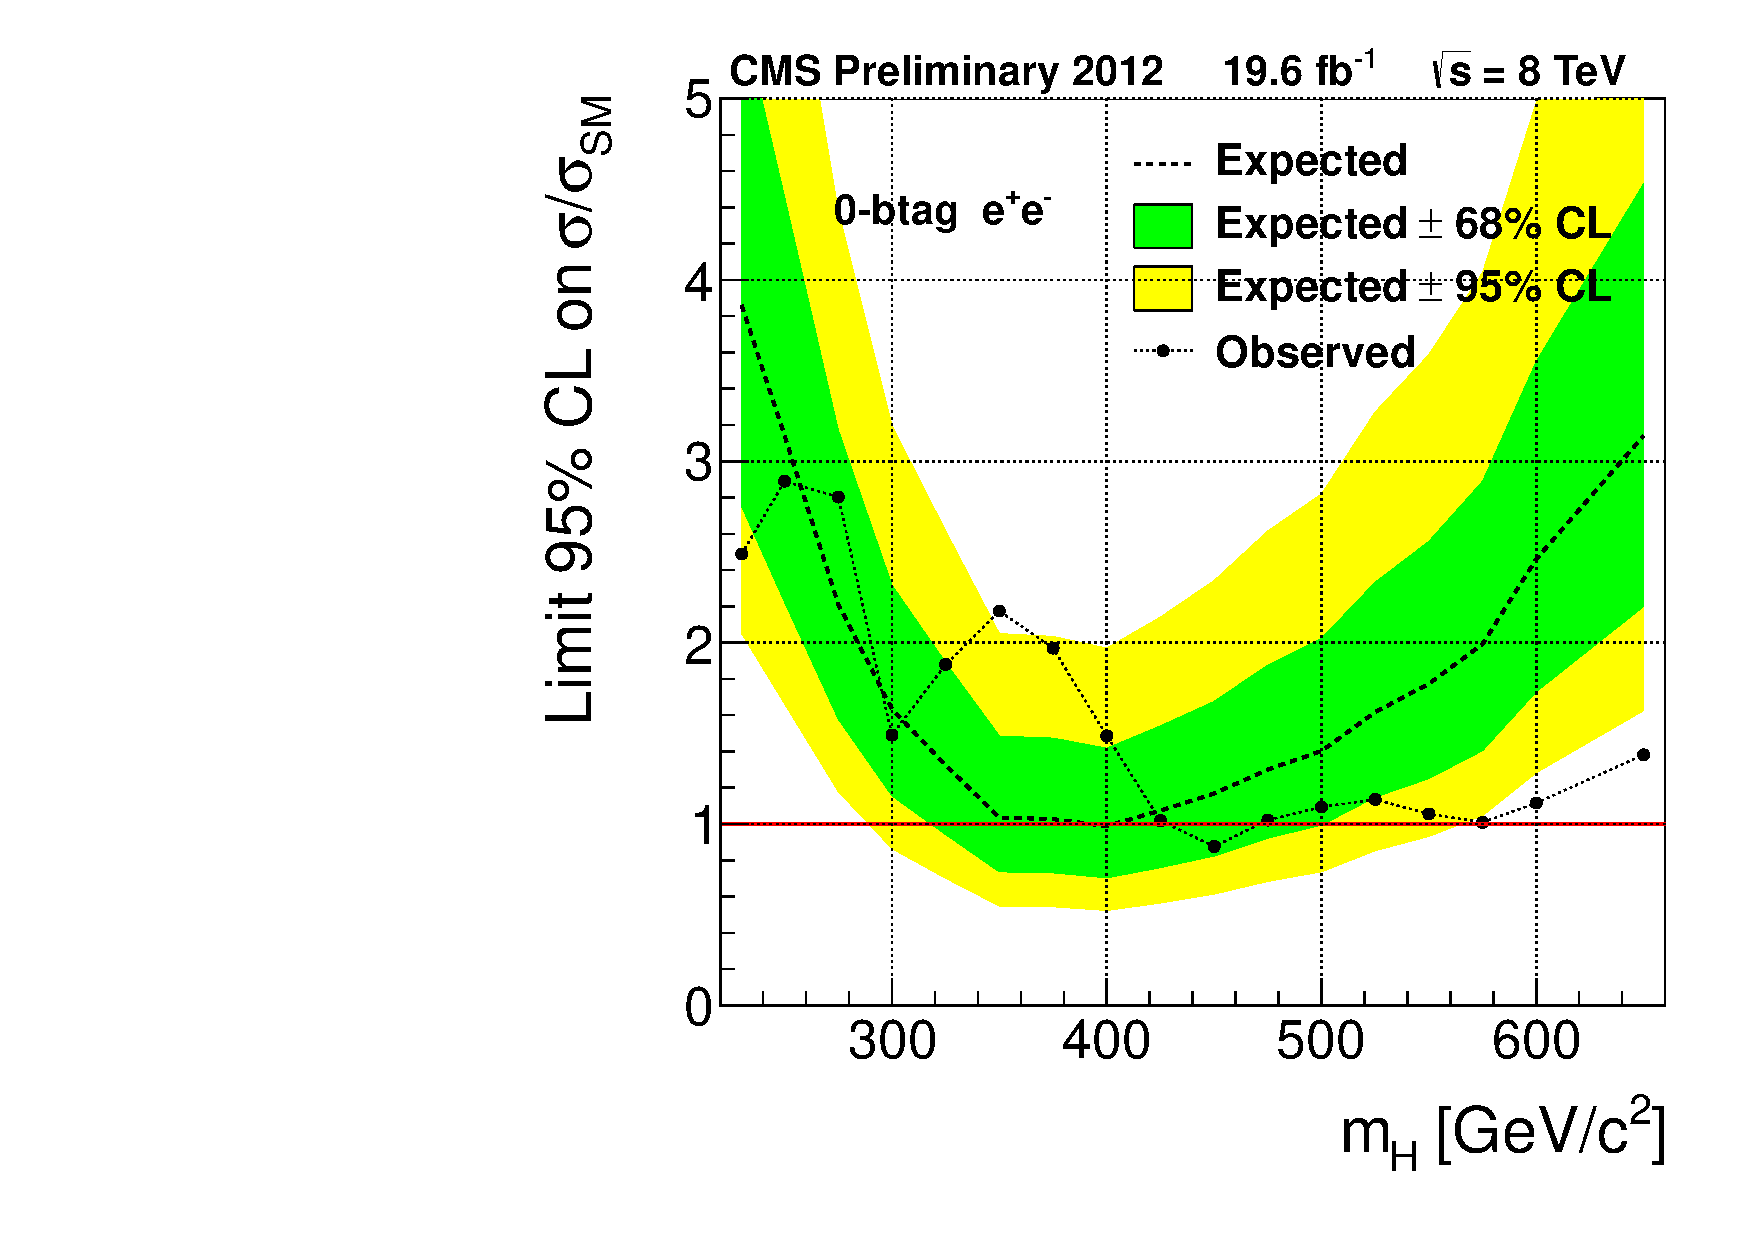
\includegraphics[width=0.33\textwidth]{plots/limit_observed_0-btag_ee.pdf}
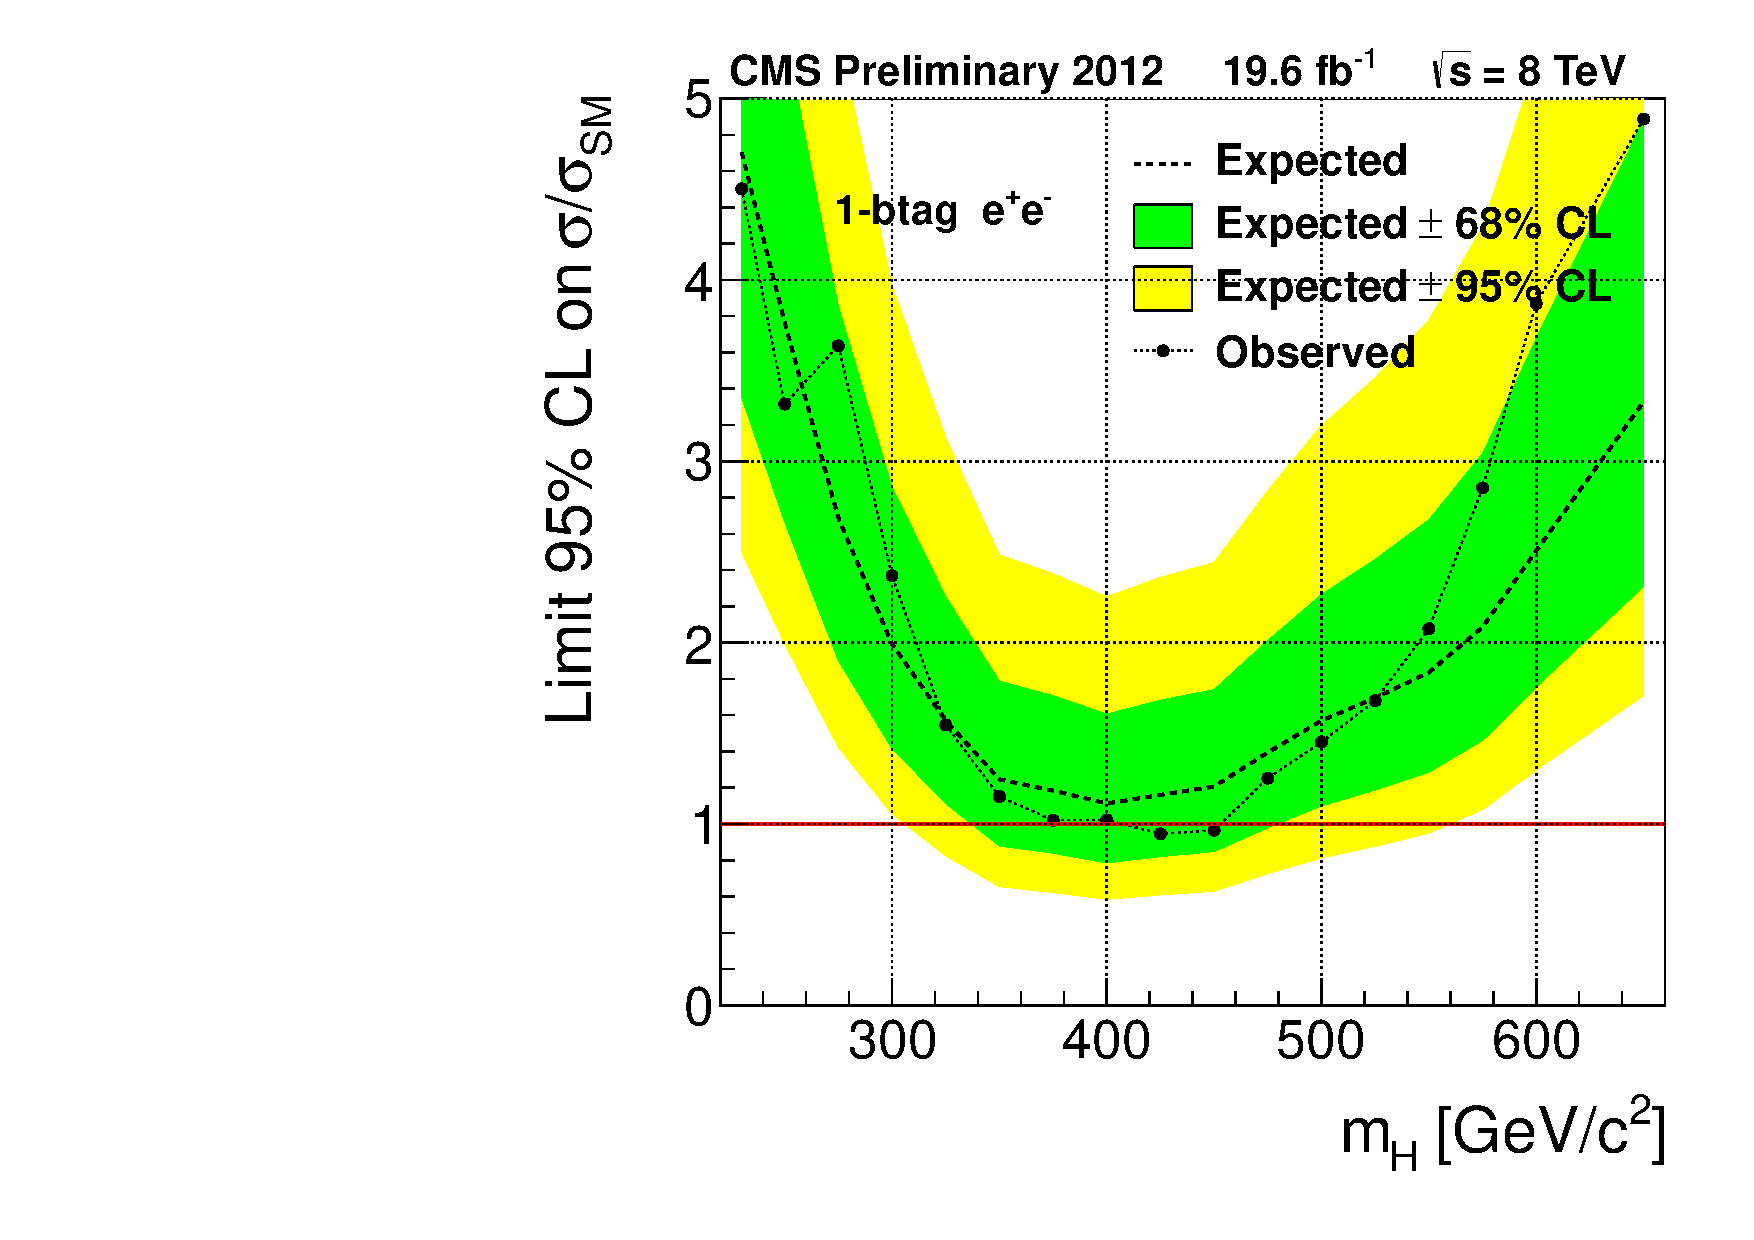
\includegraphics[width=0.33\textwidth]{plots/limit_observed_1-btag_ee.pdf}
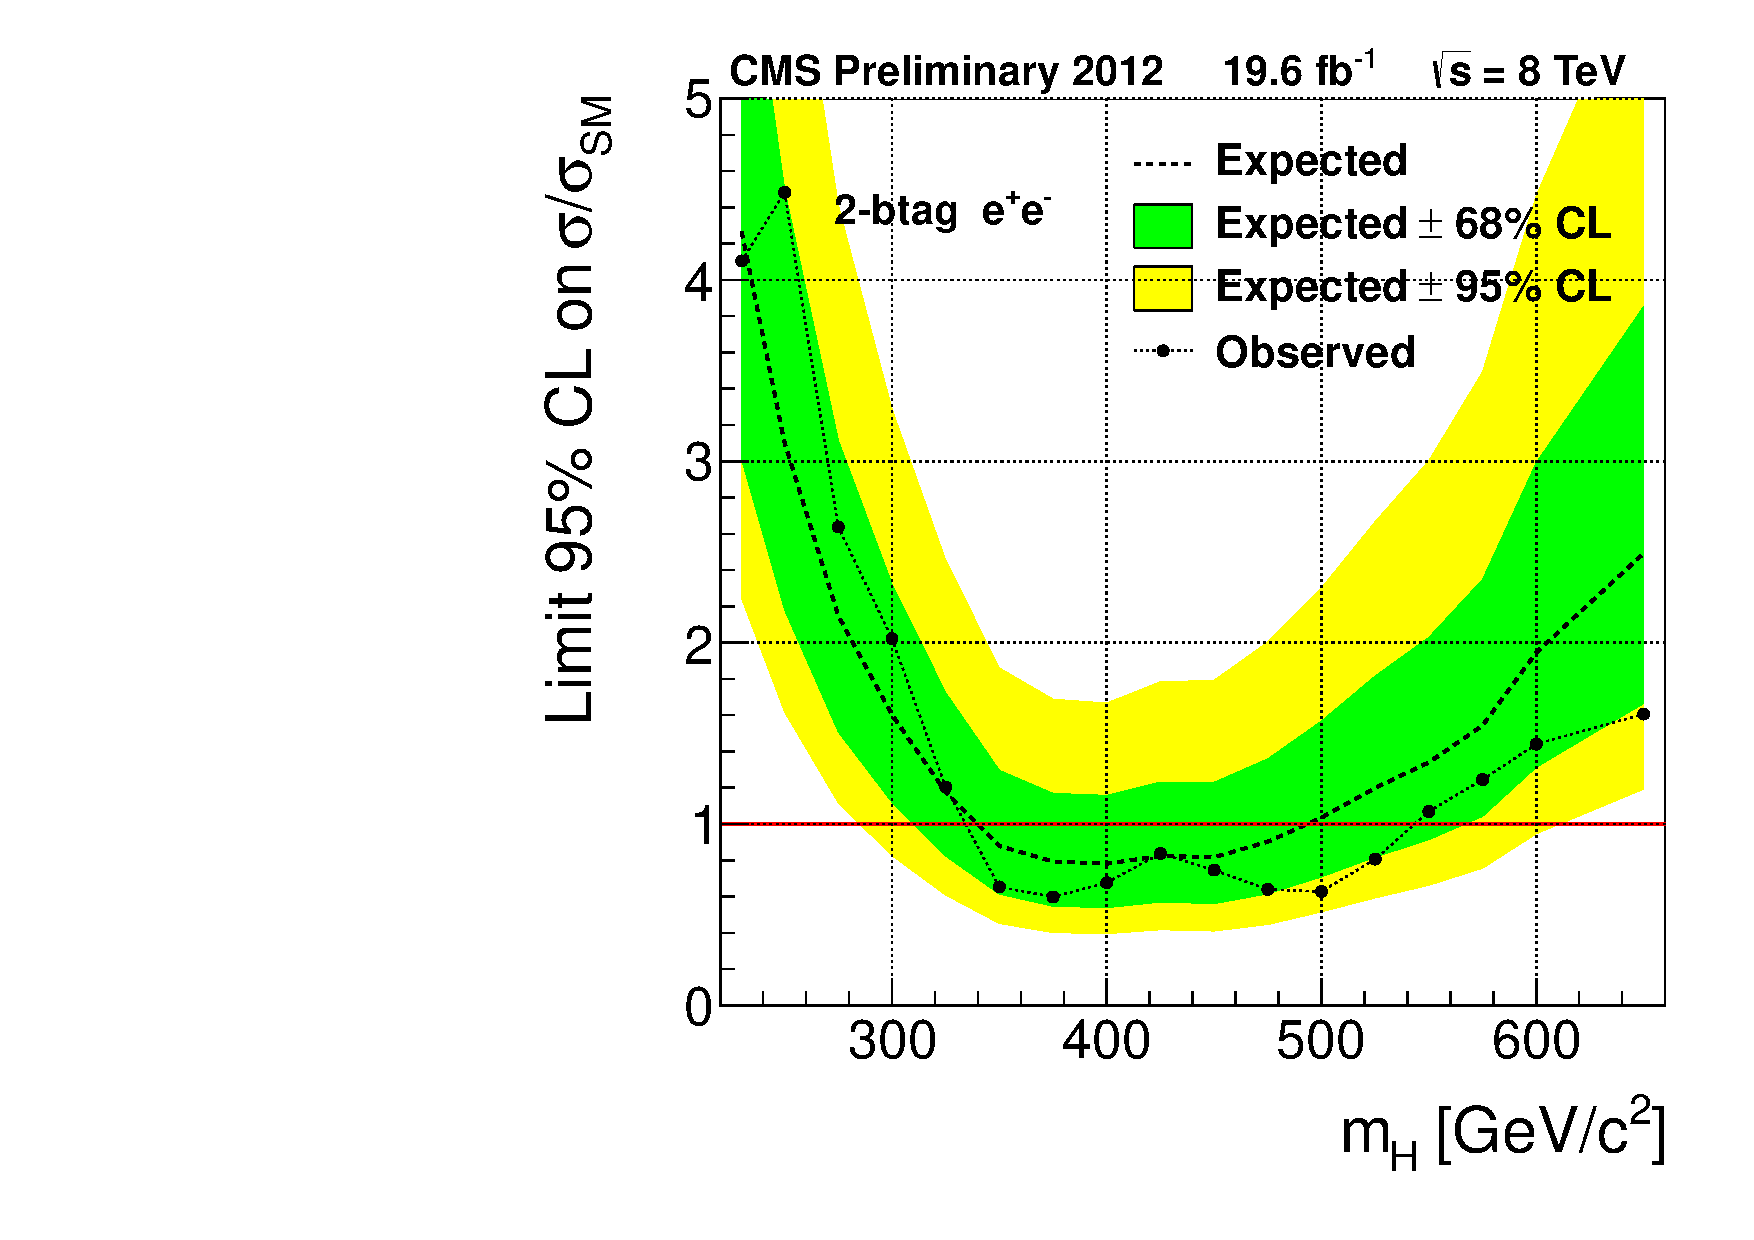
\includegraphics[width=0.33\textwidth]{plots/limit_observed_2-btag_ee.pdf}
}
\centerline{
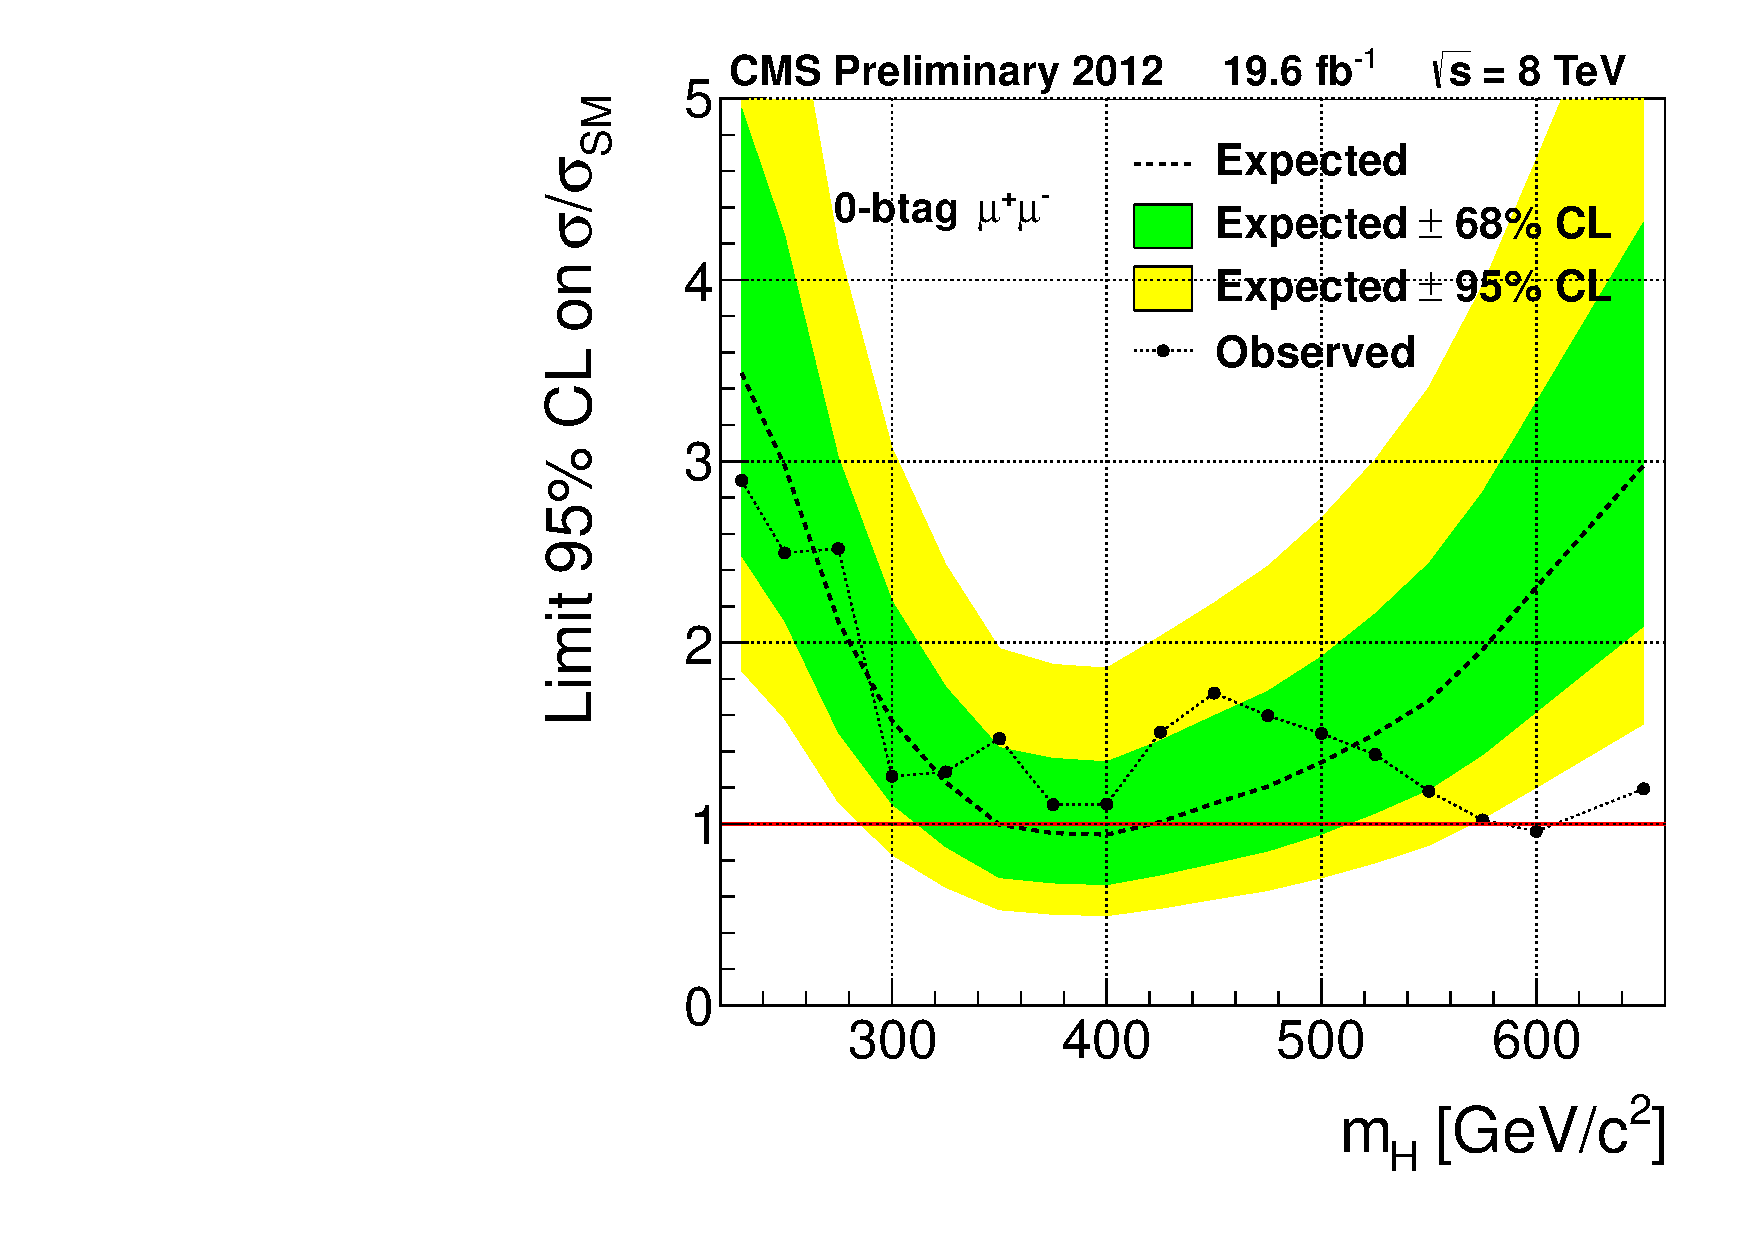
\includegraphics[width=0.33\textwidth]{plots/limit_observed_0-btag_mm.pdf}
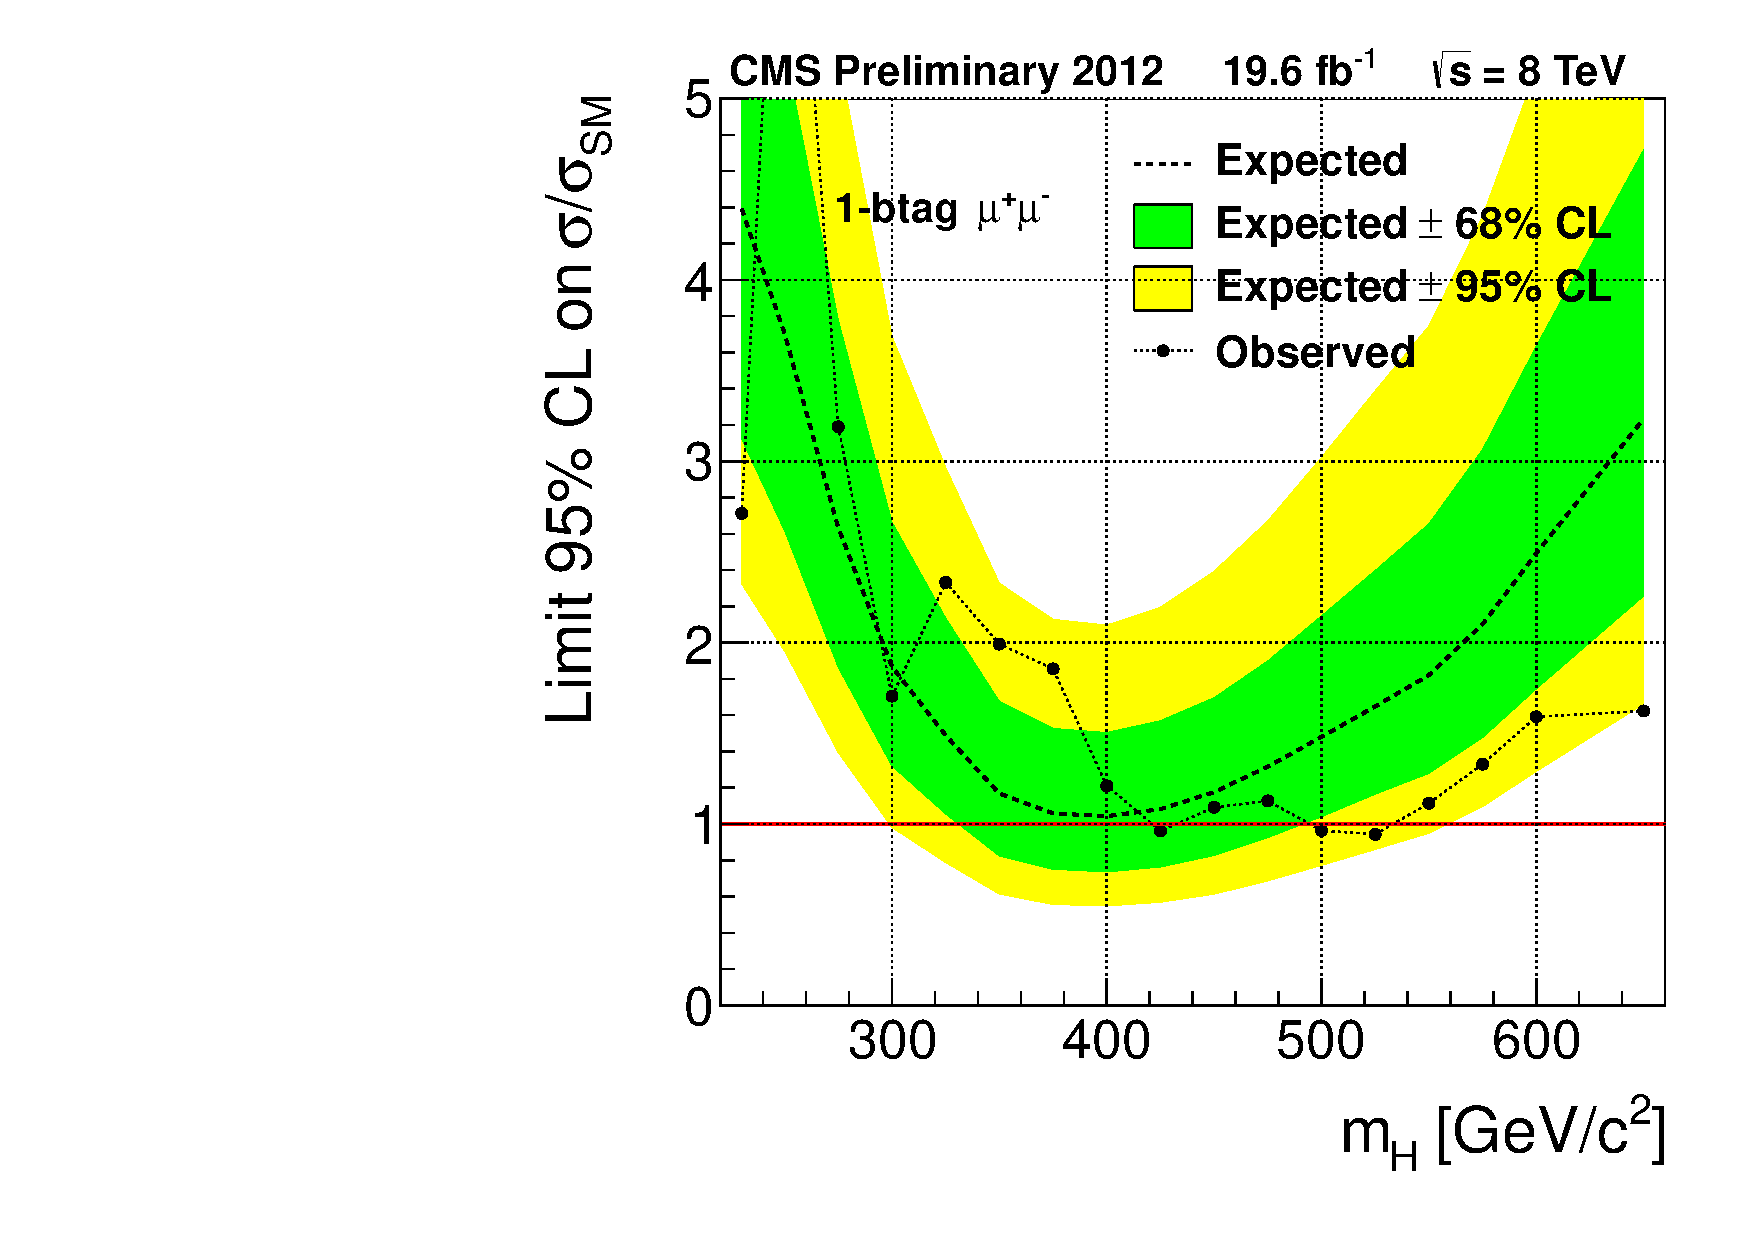
\includegraphics[width=0.33\textwidth]{plots/limit_observed_1-btag_mm.pdf}
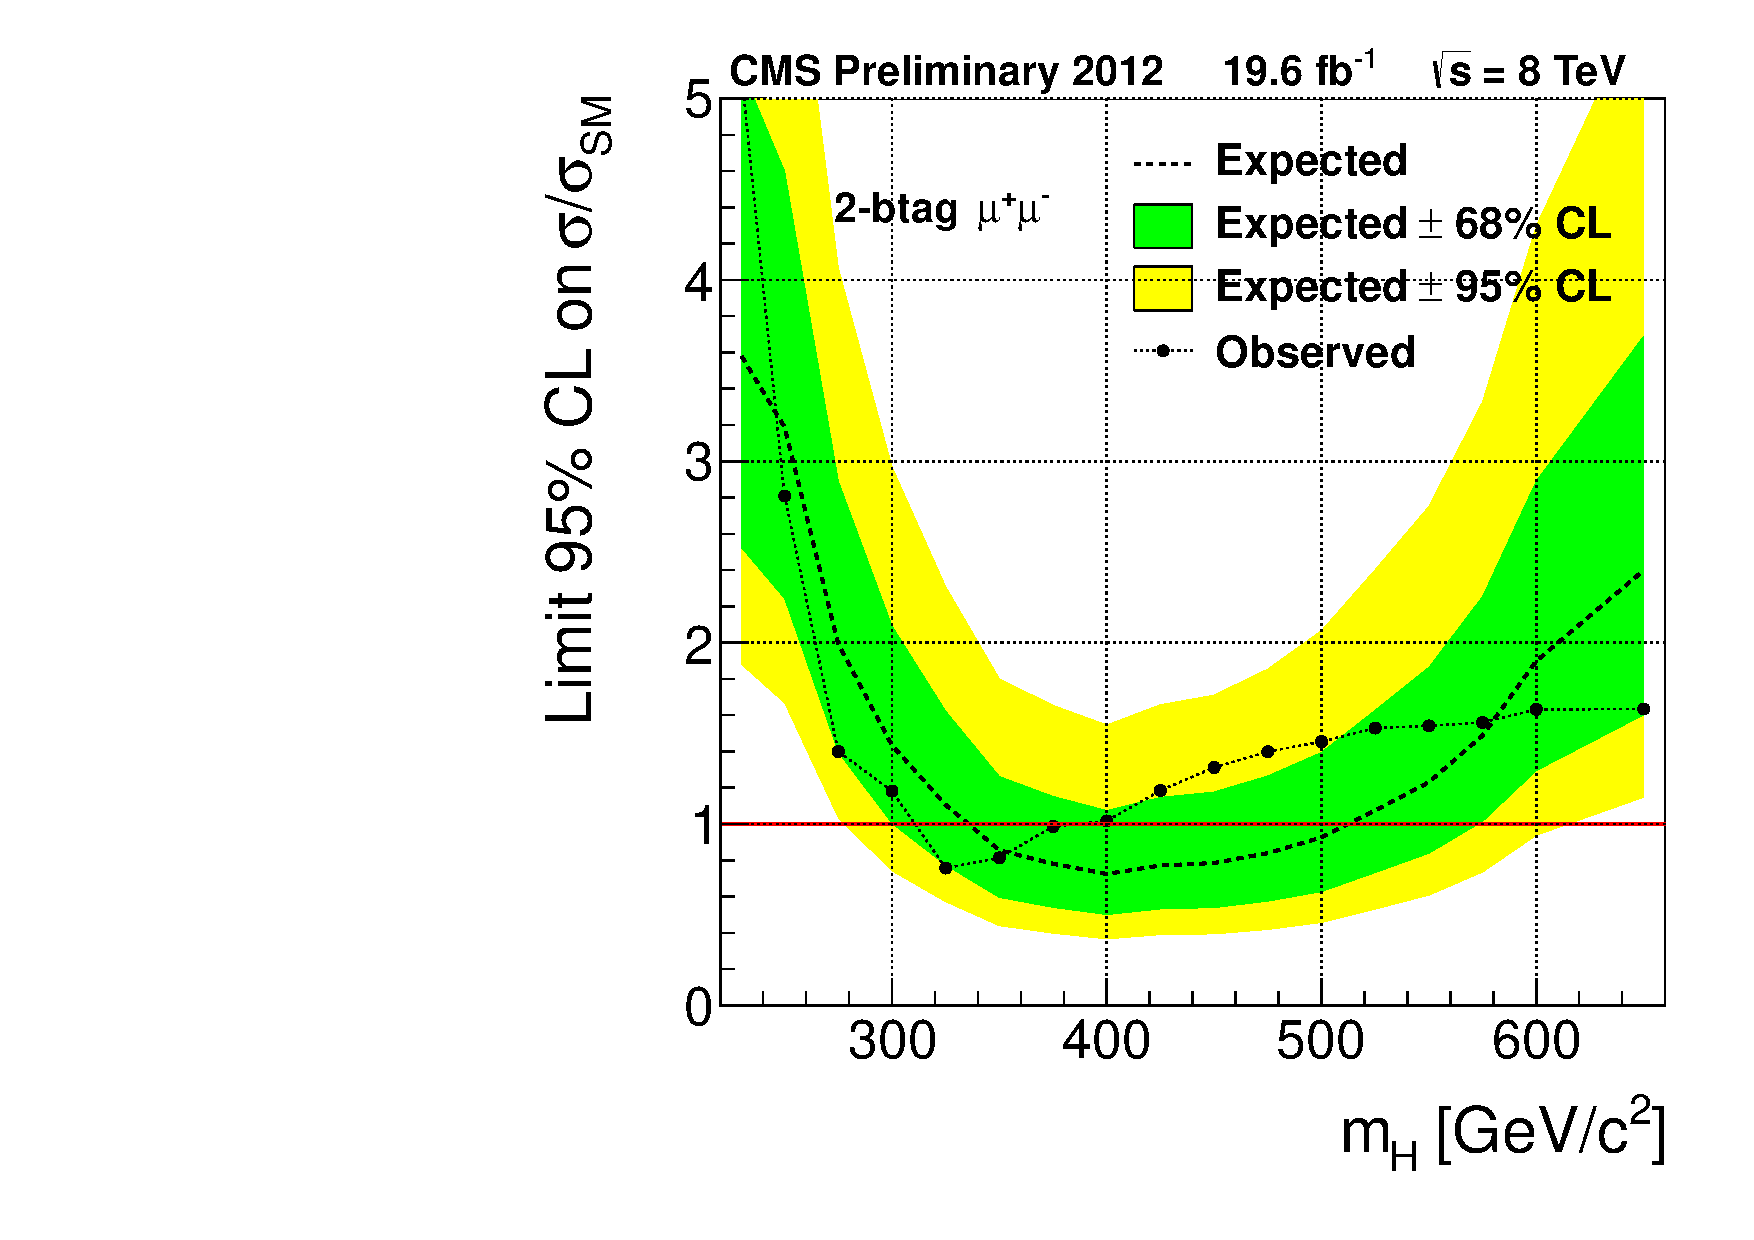
\includegraphics[width=0.33\textwidth]{plots/limit_observed_2-btag_mm.pdf}
}
\caption{
Observed (solid) and expected (dashed) 95\% CL upper limit on the ratio of the production cross section to the SM expectation for the Higgs boson obtained using the $\mathrm{CL_s}$ technique, separate for the different lepton flavor and b-tag categories. The 68\% and 95\% ranges of expectation for the background-only model are also shown with green and yellow bands, respectively.  The solid line at 1 indicates the expectation for a SM-Higgs-like boson.
}
\label{fig:limit20fb_split}
\end{center}
\end{figure}

\begin{figure}[htbp]
 \begin{center}
 \centerline{
%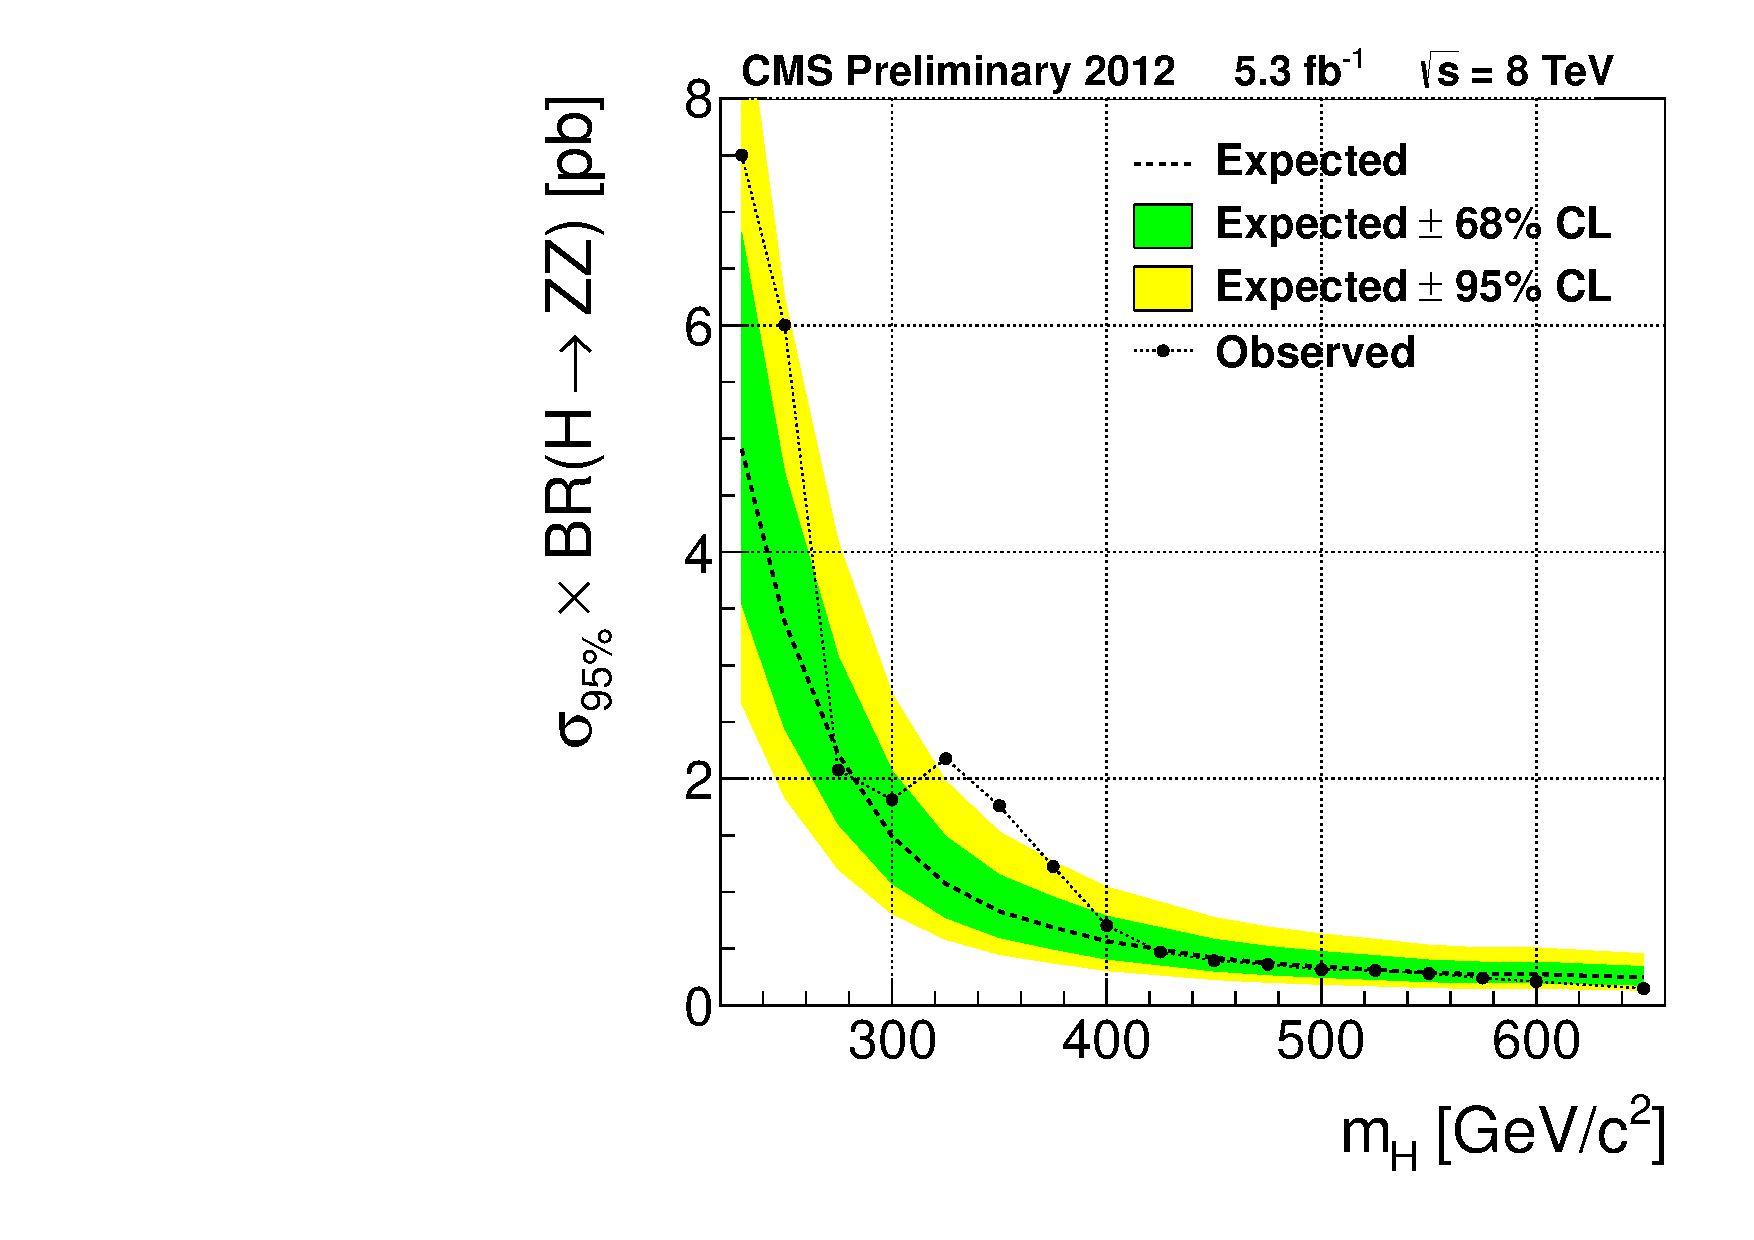
\includegraphics[width=0.49\textwidth]{plots/xs_limit_observed_all-btag_ll-ICHEP.pdf}
 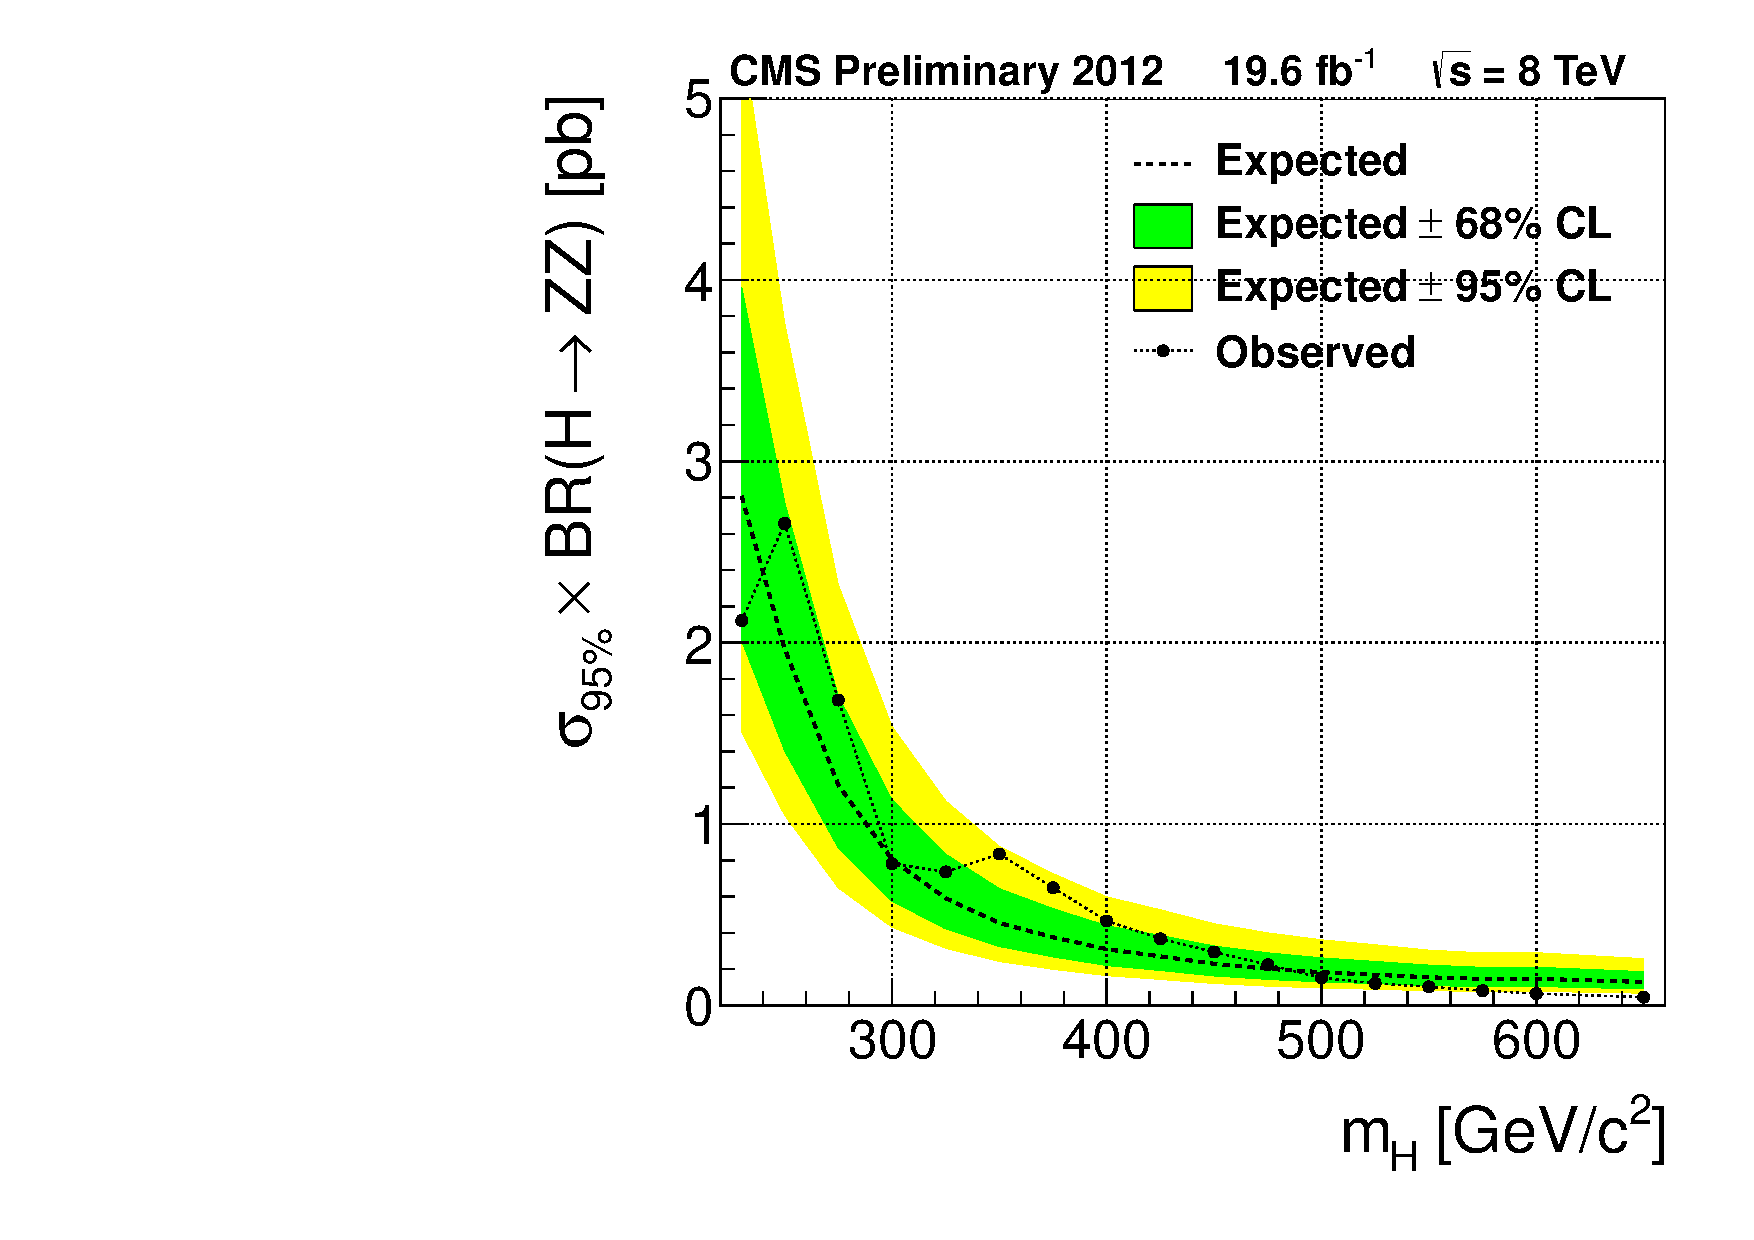
\includegraphics[width=0.79\textwidth]{plots/xs_limit_observed_all-btag_ll.pdf}
% 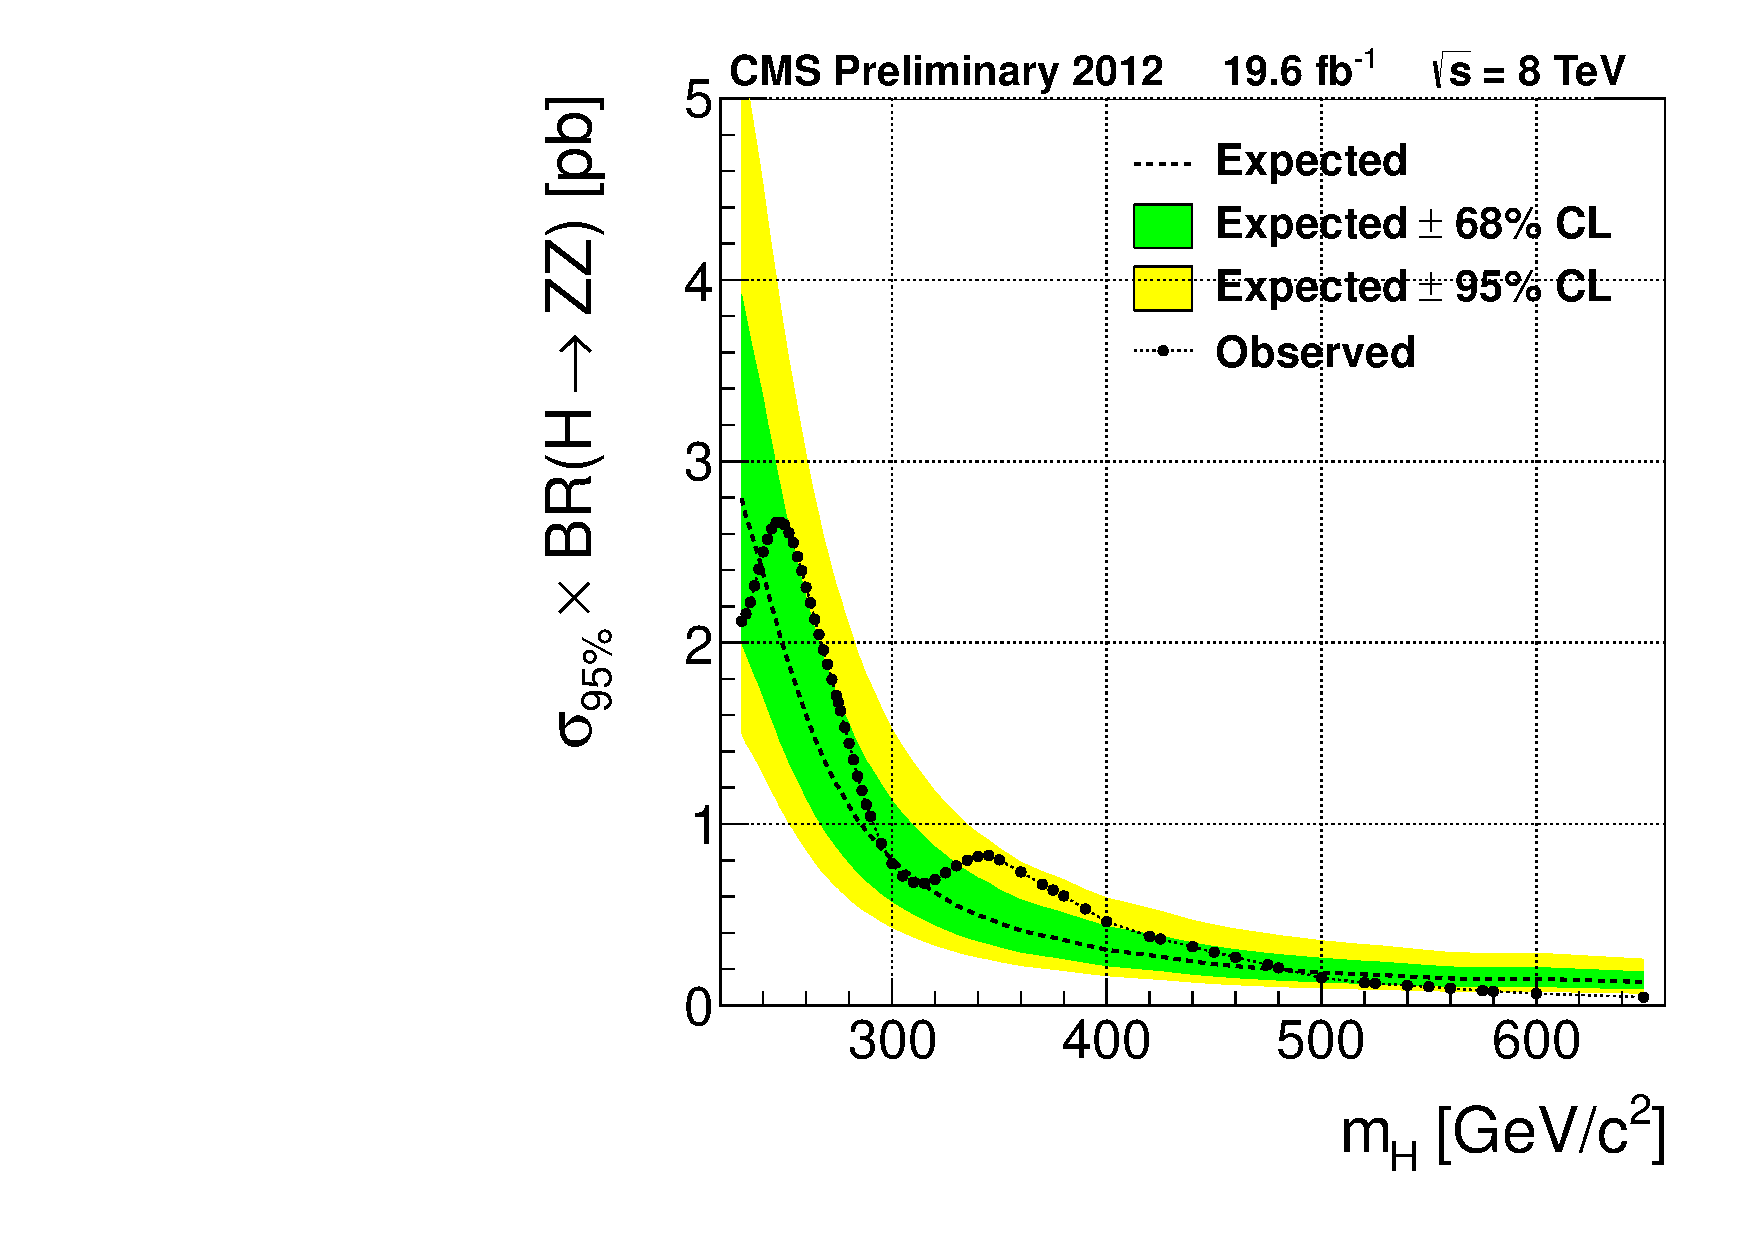
\includegraphics[width=0.49\textwidth]{plots/xs_limit_observed_all-btag_ll_inerpol.pdf}
}
\caption{
Observed (solid) and expected (dashed) 95\% C.L. upper limit on the product of the production cross section and branching fraction for $\HZZ$ obtained with the $\mathrm{CL_s}$ technique. The 68\% and 95\% ranges of expectation for the background-only model are also shown with green and yellow bands, respectively. The left plot shows the observed limit only at the points where the signal shape can be directly obtained from the simulation.
}
\label{fig:limitxs}
\end{center}
\end{figure}

%
%\begin{figure}[htbp]
%\begin{center}
%\centerline{
%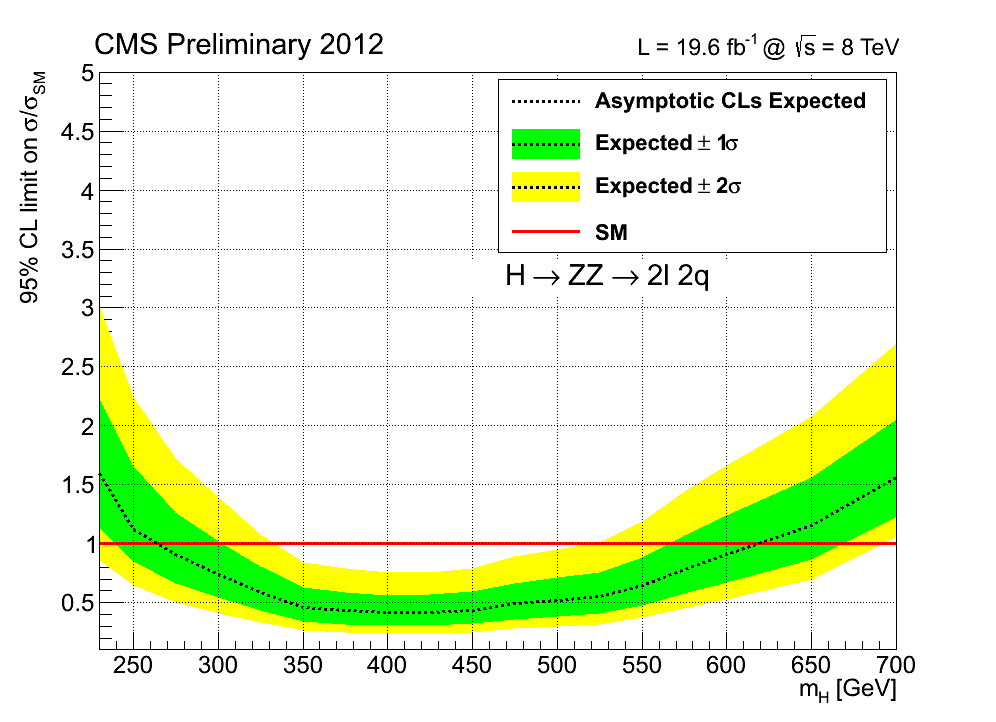
\includegraphics[width=0.55\textwidth]{plots/limit_histo_20fb_blinded.png}
%}
%\caption{
%Limit on the expected 95$\%$ CL upper limit on the product of the Higgs boson production cross sectio
%n and the branching fraction of H$\rightarrow$ZZ, using 19.6~\fbinv{} of data . Yellow and Green bands
% represent the 68$\%$ and 95$\%$ ranges of expectation.
%}
%\label{fig:limit2012}
%\end{center}
%\end{figure}

%\begin{figure}[htbp]
%\begin{center}
%\centerline{
%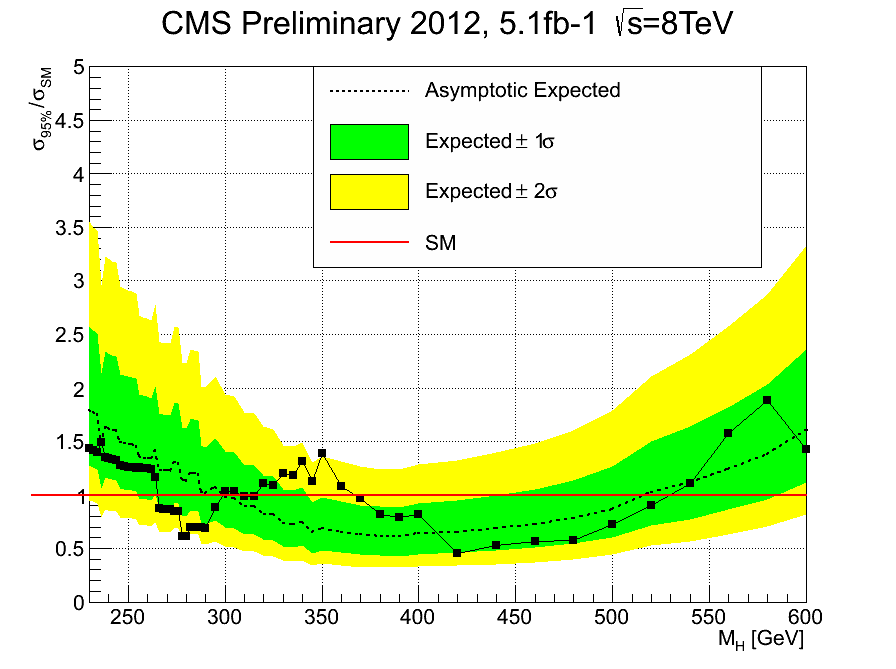
\includegraphics[width=0.49\textwidth]{plots/limit_CiC5_5fb_unblinded.png}
%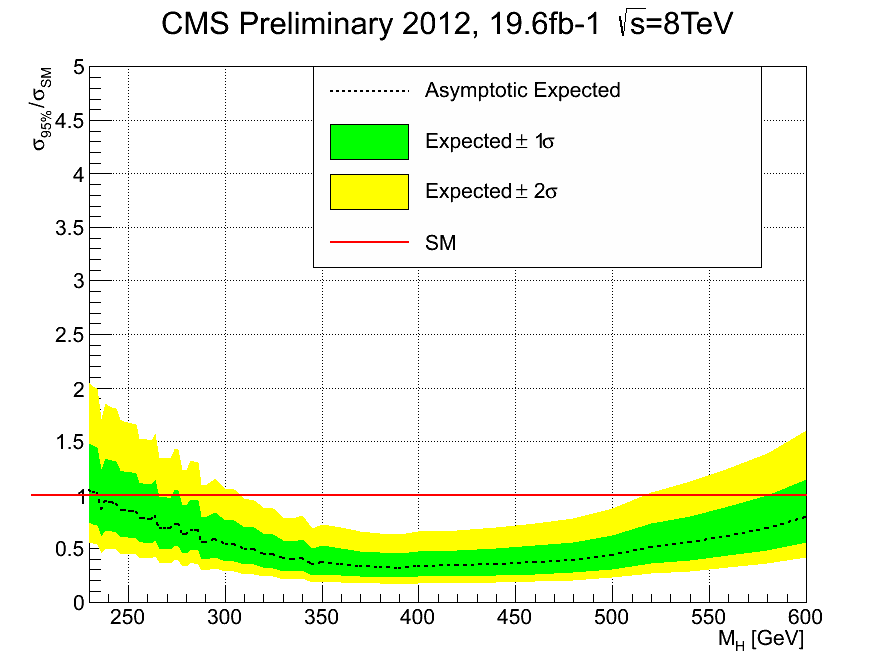
\includegraphics[width=0.49\textwidth]{plots/limit_CiC20_blinded.png}
%}
%\caption{Limit plot with the ''cut and count'' method. Color code as in Figure~\re{fig:limit5fb}.
%}
%\label{fig:limit5fbcutcount}
%\end{center}
%\end{figure}

%\begin{figure}[htbp]
%\begin{center}
%\centerline{
%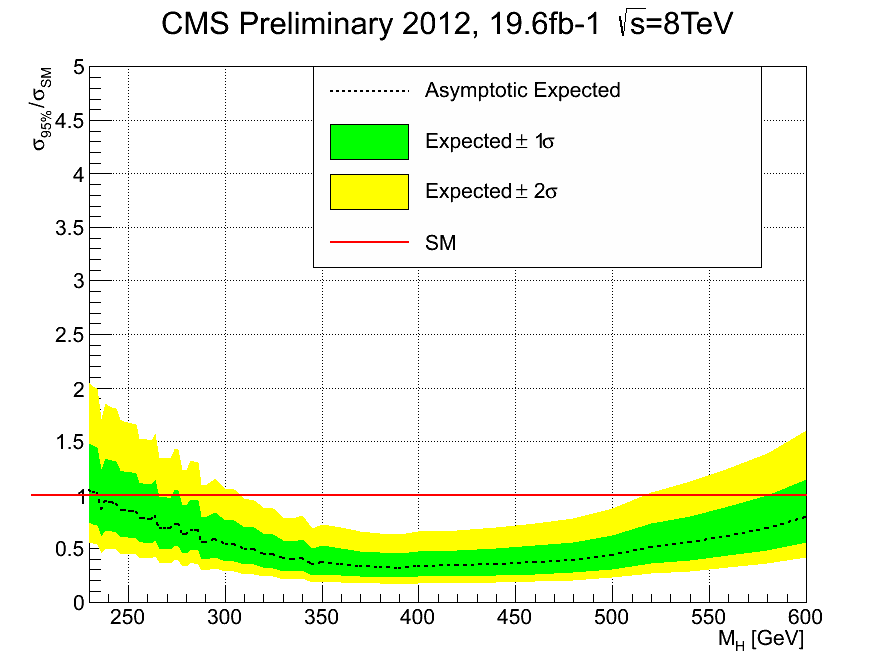
\includegraphics[width=0.55\textwidth]{plots/limit_CiC20_blinded.png}
%5}
%\caption{
%Limit on the expected 95$\%$ CL upper limit on the product of the Higgs boson production cross section
% and the branching fraction of H$\rightarrow$ZZ using 19.6~\fbinv{} of data, estimated with the ''cut and count'' method.
% Yellow and Green bands represent the 68$\%$ and 95$\%$ ranges of expectation.
%}
%\label{fig:limit2012cutcount}
%\end{center}
%\end{figure}
%


\begin{figure}[htbp]
 \centerline{
% 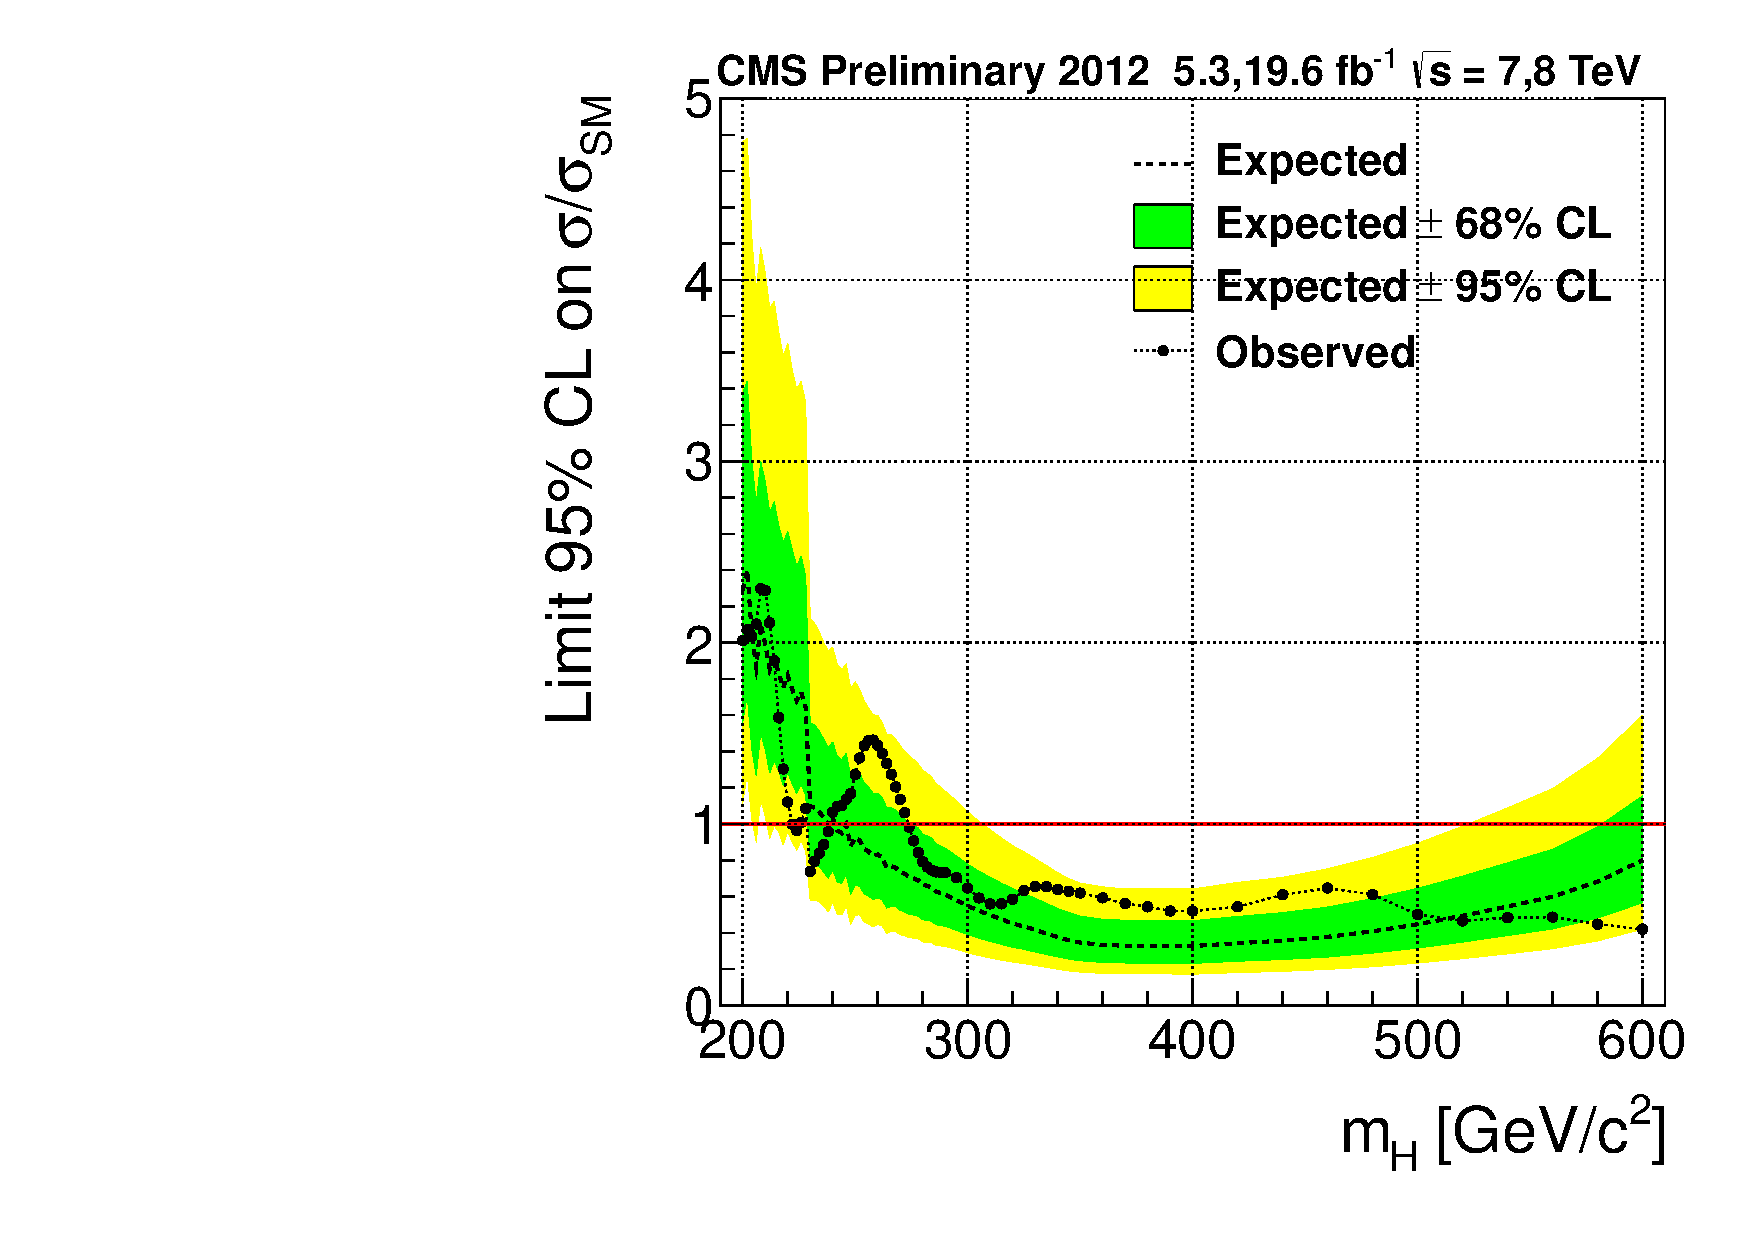
\includegraphics[width=0.6\textwidth]{plots/combined_limit_observed_all-btag_ll.pdf}
   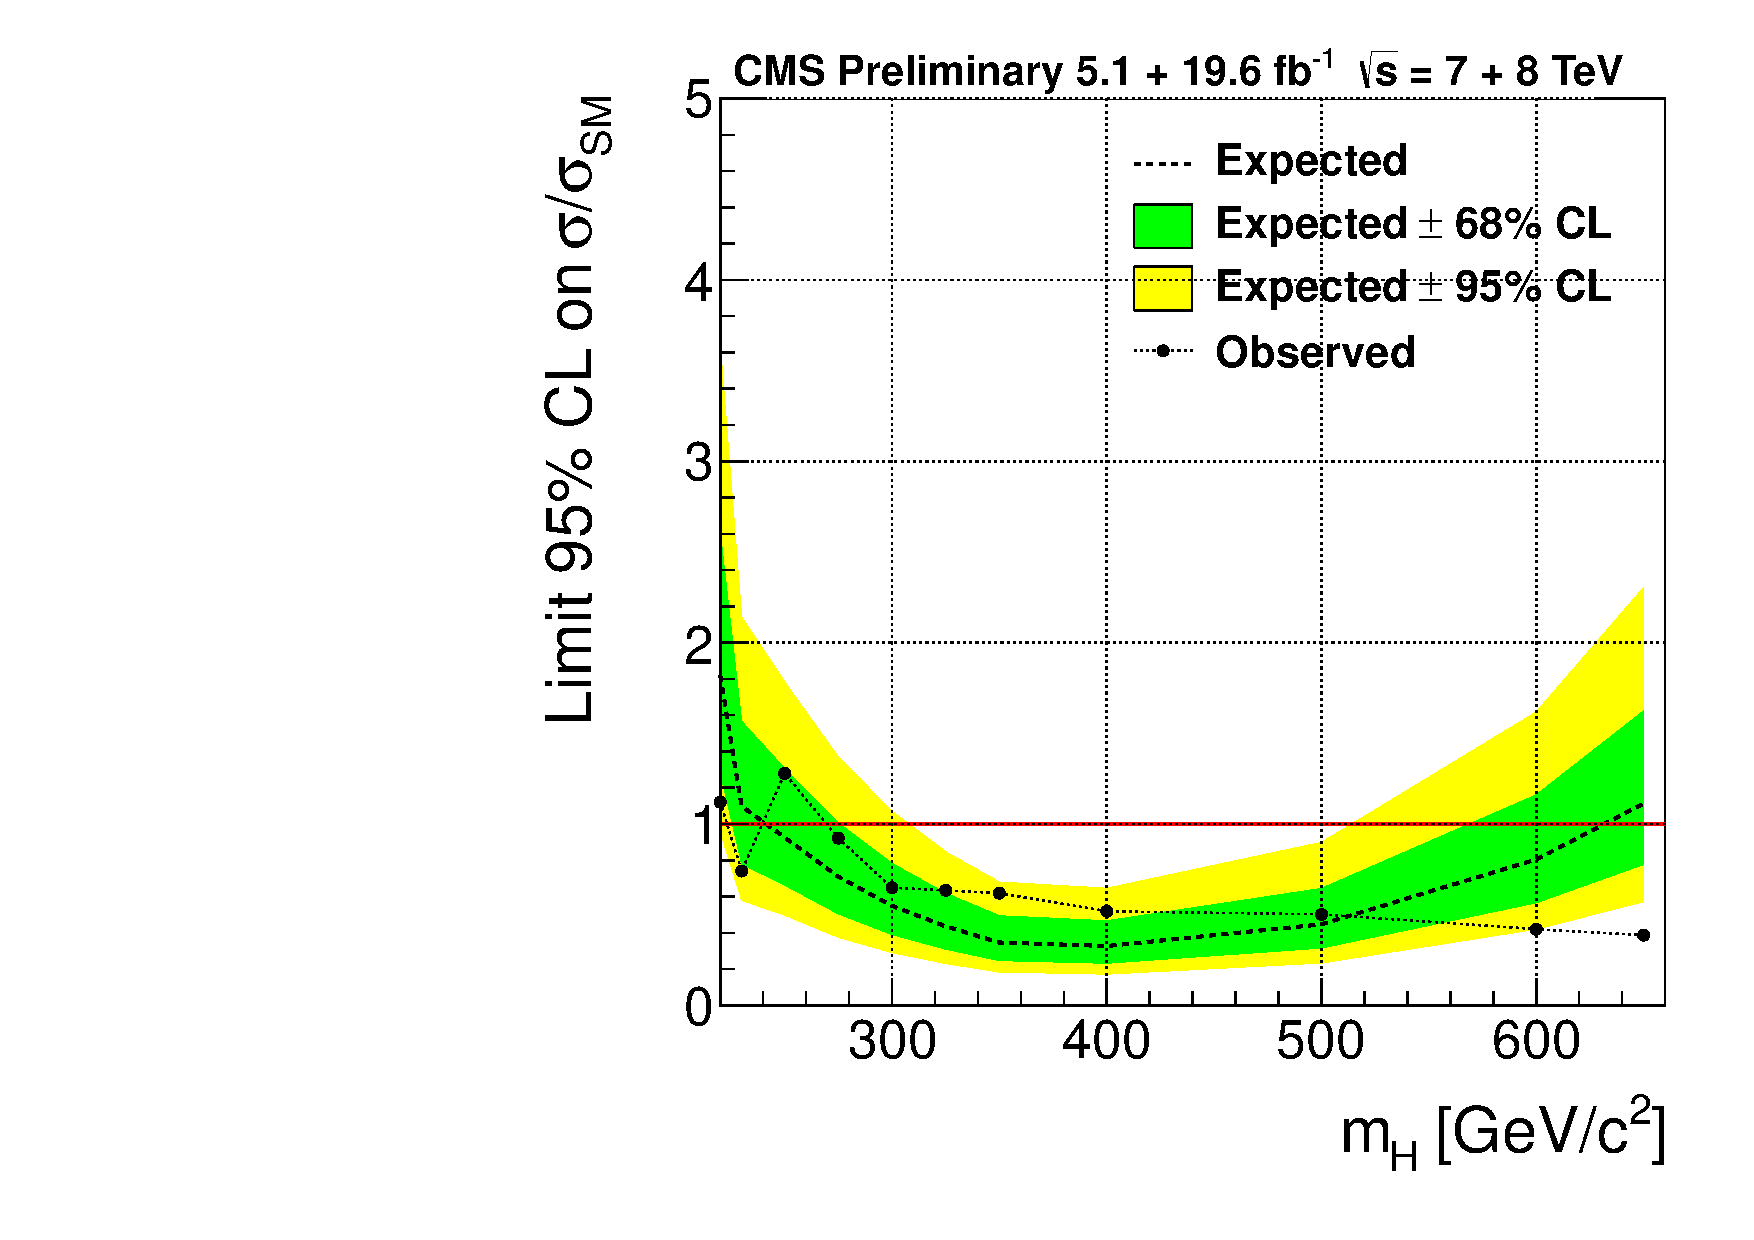
\includegraphics[width=0.79\textwidth]{plots/limit_observed_all-btag_combi.pdf}
}
 
\caption{
Observed (solid) and expected (dashed) 95\% CL upper limit on the ratio of the production cross section to the SM expectation for the Higgs boson obtained using the $\mathrm{CL_s}$ technique. The 68\% and 95\% ranges of expectation for the background-only model are also shown with green and yellow bands, respectively.  The solid line at 1 indicates the expectation for a SM-Higgs-like boson. This result is the combination of this study (i.e. Figure~\ref{fig:limit5fb}) with the previous 2011 results.
}
\label{fig:combination}
\end{figure}


